=====================================================================
%  Chapter 3: Linear Functions, Linear Transformations, and Matrices
% =====================================================================

\chapter{Linear Functions, Linear Transformations, and Matrices}
\label{ch:3}

Chapter 2 ended with the forms
\[
    dx,\qquad dy,\qquad dz,
\]
which simply read off components of a vector.  Then the wedge product used those
component readings to measure signed area and signed volume.

Now we take one step backward and ask a simpler question.  What kind of rule is
\(dx\)?  What kind of rule is \(3dx-2dy+5dz\)?  These rules take a vector as input
and return a number.  They are the first linear machines in the book.

Soon we will let a machine take a vector and return a new vector.  That is where
matrices appear.

\section{Linear functions \(\mathbb R^n\to\mathbb R\)}

Recall from Chapter 2 that
\[
    dx(x,y)=x,\qquad dy(x,y)=y,
\]
and in space,
\[
    dz(x,y,z)=z.
\]
Each of these rules measures one part of a vector.  If we double the vector, the
measurement doubles.  If we add two vectors, the measurements add.

That is the behavior we now want to name.

\subsection{A steady ramp}

Imagine a flat metal ramp in a warehouse.  Moving one meter east raises you \(3\) cm.
Moving one meter north raises you \(2\) cm.

If your displacement along the floor is
\[
    \mathbf v=(x,y),
\]
then your change in height is
\[
    L(x,y)=3x+2y.
\]
For example,
\[
    L(4,-1)=3\cdot4+2(-1)=10.
\]
So moving \(4\) meters east and \(1\) meter south raises you \(10\) cm.

This rule has two very natural properties.

First, if you break a trip into two pieces,
\[
    \mathbf u=(x_1,y_1),
    \qquad
    \mathbf v=(x_2,y_2),
\]
then
\[
\begin{aligned}
L(\mathbf u+\mathbf v)
&=
L(x_1+x_2,y_1+y_2)\\
&=
3(x_1+x_2)+2(y_1+y_2)\\
&=
(3x_1+2y_1)+(3x_2+2y_2)\\
&=
L(\mathbf u)+L(\mathbf v).
\end{aligned}
\]
The height gained on the whole trip is the sum of the height gains on the pieces.

Second, if you stretch a displacement by a factor \(c\), the height change stretches by
the same factor:
\[
\begin{aligned}
L(c\mathbf u)
&=
L(cx_1,cy_1)\\
&=
3cx_1+2cy_1\\
&=
c(3x_1+2y_1)\\
&=
cL(\mathbf u).
\end{aligned}
\]

These two properties are what linearity means.

\begin{definition}[Linear function]
A function
\[
    \ell:\mathbb R^n\to\mathbb R
\]
is called \emph{linear} if, for all vectors \(\mathbf u,\mathbf v\in\mathbb R^n\)
and all scalars \(c\),
\[
    \ell(\mathbf u+\mathbf v)=\ell(\mathbf u)+\ell(\mathbf v),
\]
and
\[
    \ell(c\mathbf u)=c\ell(\mathbf u).
\]
\end{definition}

The two rules can be combined.  If \(\ell\) is linear, then
\[
    \ell(a\mathbf u+b\mathbf v)
    =
    a\ell(\mathbf u)+b\ell(\mathbf v).
\]
More generally,
\[
    \ell(c_1\mathbf v_1+\cdots+c_k\mathbf v_k)
    =
    c_1\ell(\mathbf v_1)+\cdots+c_k\ell(\mathbf v_k).
\]

A linear function must also send the zero vector to zero:
\[
    \ell(\mathbf 0)=0.
\]
Indeed,
\[
    \ell(\mathbf 0)=\ell(0\mathbf u)=0\ell(\mathbf u)=0.
\]

This small fact is a useful warning.

\begin{example}[A rule that is almost linear but not linear]
The rule
\[
    A(x,y)=3x+2y+10
\]
looks very much like the ramp rule, but it is not linear.  It does not send the zero
vector to zero:
\[
    A(0,0)=10.
\]
It describes a flat ramp whose height at the origin is already \(10\) cm.  Such rules are
called \emph{affine}.  They will matter later, especially for tangent planes.  But they
are not linear.
\end{example}

\begin{example}[A rule that bends]
The rule
\[
    Q(x,y)=x^2+y
\]
is not linear.  For instance,
\[
    Q(2,0)=4,
\]
but
\[
    2Q(1,0)=2.
\]
Doubling the input did not double the output.  The square term bends the rule.
\end{example}

Linear functions are the rules that do not bend and do not shift the origin.

\subsection{Values on basis vectors determine the whole function}

The ramp rule
\[
    L(x,y)=3x+2y
\]
is completely determined by what it does to the two standard basis vectors:
\[
    \mathbf e_1=(1,0),
    \qquad
    \mathbf e_2=(0,1).
\]
Indeed,
\[
    L(\mathbf e_1)=3,
    \qquad
    L(\mathbf e_2)=2.
\]
Since every vector in \(\mathbb R^2\) can be written as
\[
    (x,y)=x\mathbf e_1+y\mathbf e_2,
\]
linearity forces
\[
\begin{aligned}
L(x,y)
&=
L(x\mathbf e_1+y\mathbf e_2)\\
&=
xL(\mathbf e_1)+yL(\mathbf e_2)\\
&=
3x+2y.
\end{aligned}
\]

So once we know the two numbers
\[
    L(\mathbf e_1),\qquad L(\mathbf e_2),
\]
we know \(L\) everywhere.

The same idea works in every dimension.

\begin{theorem}[A linear function is determined by its values on the standard basis]
Let
\[
    \ell:\mathbb R^n\to\mathbb R
\]
be linear.  If
\[
    \mathbf e_1,\mathbf e_2,\ldots,\mathbf e_n
\]
are the standard basis vectors, then every vector
\[
    \mathbf x=(x_1,x_2,\ldots,x_n)
\]
satisfies
\[
\boxed{
    \ell(\mathbf x)
    =
    x_1\ell(\mathbf e_1)+x_2\ell(\mathbf e_2)+\cdots+x_n\ell(\mathbf e_n).
}
\]
\end{theorem}

\begin{proof}
Every vector in \(\mathbb R^n\) can be written as
\[
    \mathbf x=x_1\mathbf e_1+x_2\mathbf e_2+\cdots+x_n\mathbf e_n.
\]
Using linearity,
\[
\begin{aligned}
\ell(\mathbf x)
&=
\ell(x_1\mathbf e_1+x_2\mathbf e_2+\cdots+x_n\mathbf e_n)\\
&=
x_1\ell(\mathbf e_1)+x_2\ell(\mathbf e_2)+\cdots+x_n\ell(\mathbf e_n).
\end{aligned}
\]
\end{proof}

This theorem is one of the main reasons basis vectors are useful.  To understand a
linear rule, we do not have to test every vector.  We only test the basic directions.

\subsection{Linear functions as dot products with fixed vectors}

Suppose a small cart moves through space by
\[
    \mathbf x=(x,y,z)
\]
meters, and a constant force
\[
    \mathbf F=(6,-2,4)
\]
newtons acts on it.  The work done by the force is
\[
    W(x,y,z)=6x-2y+4z.
\]
This is a linear function:
\[
    W:\mathbb R^3\to\mathbb R.
\]
It is also a dot product:
\[
    W(\mathbf x)=\mathbf F\cdot\mathbf x.
\]

This was the first physical reason for the dot product in Chapter 2.  Now it becomes a
general algebraic fact: every linear function is a dot product with one fixed vector.

For vectors in \(\mathbb R^n\), we use the same dot product formula:
\[
    \mathbf a\cdot\mathbf x
    =
    a_1x_1+a_2x_2+\cdots+a_nx_n.
\]

\begin{theorem}[Every linear function is a dot product]
Let
\[
    \ell:\mathbb R^n\to\mathbb R
\]
be linear.  Then there is a unique vector
\[
    \mathbf a=(a_1,a_2,\ldots,a_n)
\]
such that
\[
\boxed{
    \ell(\mathbf x)=\mathbf a\cdot\mathbf x
}
\]
for every \(\mathbf x\in\mathbb R^n\).

The vector is
\[
\boxed{
    \mathbf a=
    \bigl(\ell(\mathbf e_1),\ell(\mathbf e_2),\ldots,\ell(\mathbf e_n)\bigr).
}
\]
\end{theorem}

\begin{proof}
Set
\[
    a_1=\ell(\mathbf e_1),\quad
    a_2=\ell(\mathbf e_2),\quad
    \ldots,\quad
    a_n=\ell(\mathbf e_n).
\]
For
\[
    \mathbf x=(x_1,\ldots,x_n),
\]
the previous theorem gives
\[
\begin{aligned}
\ell(\mathbf x)
&=
x_1\ell(\mathbf e_1)+\cdots+x_n\ell(\mathbf e_n)\\
&=
a_1x_1+\cdots+a_nx_n\\
&=
\mathbf a\cdot\mathbf x.
\end{aligned}
\]

The vector \(\mathbf a\) is unique because its components are forced:
\[
    a_j=\mathbf a\cdot\mathbf e_j=\ell(\mathbf e_j).
\]
\end{proof}

\begin{example}[Finding the fixed vector]
Let
\[
    \ell:\mathbb R^3\to\mathbb R
\]
be linear, and suppose
\[
    \ell(\mathbf e_1)=5,\qquad
    \ell(\mathbf e_2)=-1,\qquad
    \ell(\mathbf e_3)=4.
\]
Then
\[
    \ell(x,y,z)=5x-y+4z.
\]
Equivalently,
\[
    \ell(\mathbf x)=(5,-1,4)\cdot\mathbf x.
\]

For example,
\[
    \ell(2,3,-1)
    =
    5\cdot2-3+4(-1)
    =
    3.
\]
\end{example}

The fixed vector
\[
    \mathbf a
\]
is the coefficient vector of the linear function.  It tells us how strongly the function
measures each coordinate direction.

\subsection{Level sets of linear functions}

Return to the ramp
\[
    L(x,y)=3x+2y.
\]
The set of all displacements that produce height change \(12\) cm is
\[
    3x+2y=12.
\]
This is a line.

The set of all displacements that produce height change \(0\) is
\[
    3x+2y=0.
\]
This is the line of level motion along the ramp.  Walking in such a direction does not
raise or lower you.

\begin{figure}[H]
\centering
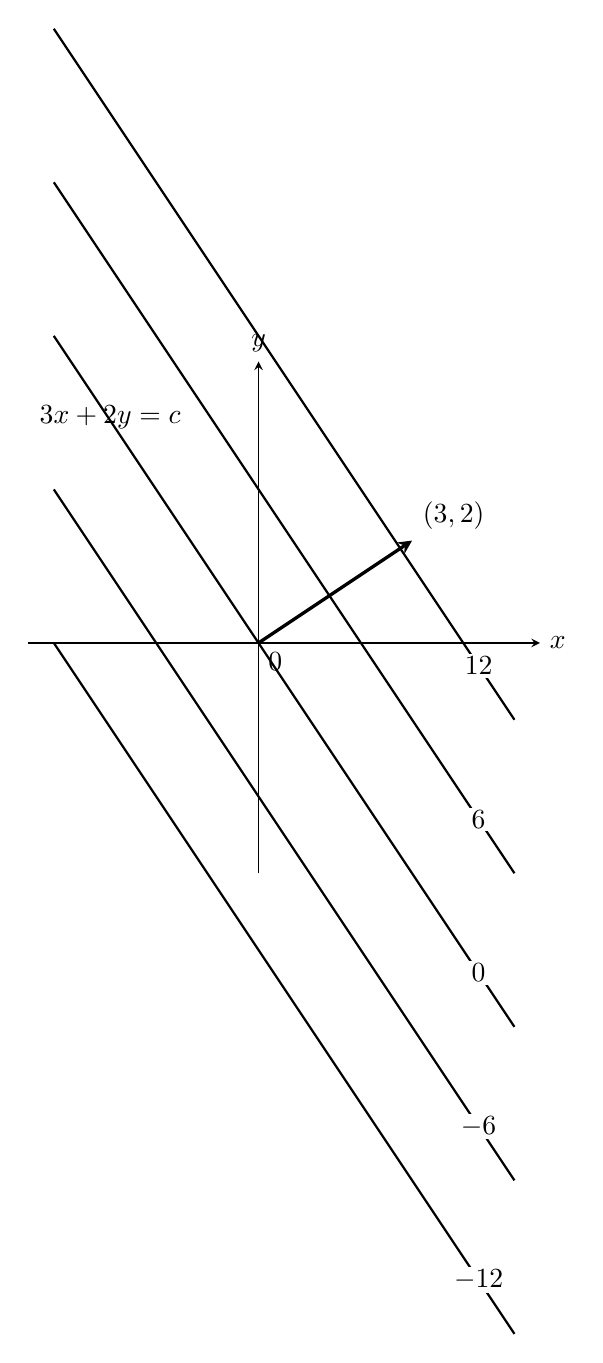
\begin{tikzpicture}[scale=0.65, >=stealth]
    \draw[->] (-4.5,0) -- (5.5,0) node[right] {\(x\)};
    \draw[->] (0,-4.5) -- (0,5.5) node[above] {\(y\)};

    \foreach \c/\lab in {-12/{-12}, -6/{-6}, 0/{0}, 6/{6}, 12/{12}} {
        \draw[thick] (-4,{(\c-3*(-4))/2}) -- (5,{(\c-3*5)/2});
        \node[fill=white, inner sep=1pt] at (4.3,{(\c-3*4.3)/2}) {\(\lab\)};
    }

    \draw[->, very thick] (0,0) -- (3,2) node[above right] {\((3,2)\)};
    \node at (-2.9,4.4) {\(3x+2y=c\)};
    \node[below right] at (0,0) {\(0\)};
\end{tikzpicture}
\caption{The level sets of \(L(x,y)=3x+2y\) are parallel lines.  The vector \((3,2)\)
is perpendicular to them.}
\end{figure}

The coefficient vector
\[
    \mathbf a=(3,2)
\]
is perpendicular to these level lines.  To see why, take two points \(\mathbf p\) and
\(\mathbf q\) on the same level set:
\[
    \mathbf a\cdot\mathbf p=c,
    \qquad
    \mathbf a\cdot\mathbf q=c.
\]
Subtract:
\[
    \mathbf a\cdot(\mathbf p-\mathbf q)=0.
\]
So every displacement \(\mathbf p-\mathbf q\) along the level set is orthogonal to
\(\mathbf a\).

The same idea works in space.  A linear function
\[
    \ell(x,y,z)=ax+by+cz
\]
has level sets
\[
    ax+by+cz=d.
\]
When \((a,b,c)\neq(0,0,0)\), these are planes.  The vector
\[
    (a,b,c)
\]
is normal to the planes.

\begin{theorem}[Level sets of a nonzero linear function]
Let
\[
    \ell(\mathbf x)=\mathbf a\cdot\mathbf x
\]
be a linear function on \(\mathbb R^n\), with
\[
    \mathbf a\neq\mathbf 0.
\]
For each number \(c\), the level set
\[
    \ell(\mathbf x)=c
\]
is an affine hyperplane.  Its direction vectors are precisely the vectors
\[
    \mathbf w
\]
that satisfy
\[
    \mathbf a\cdot\mathbf w=0.
\]
\end{theorem}

\begin{proof}
Because \(\mathbf a\neq\mathbf 0\), the point
\[
    \mathbf p=\frac{c}{\|\mathbf a\|^2}\mathbf a
\]
satisfies
\[
    \mathbf a\cdot\mathbf p
    =
    \mathbf a\cdot\left(\frac{c}{\|\mathbf a\|^2}\mathbf a\right)
    =
    \frac{c}{\|\mathbf a\|^2}(\mathbf a\cdot\mathbf a)
    =
    c.
\]
So the level set is not empty.

Now a point \(\mathbf x\) lies on the same level set exactly when
\[
    \mathbf a\cdot\mathbf x=c.
\]
Since
\[
    \mathbf a\cdot\mathbf p=c,
\]
this is equivalent to
\[
    \mathbf a\cdot(\mathbf x-\mathbf p)=0.
\]
Thus
\[
    \mathbf x=\mathbf p+\mathbf w,
    \qquad
    \text{where }
    \mathbf a\cdot\mathbf w=0.
\]
That is an affine hyperplane through \(\mathbf p\), with direction space perpendicular
to \(\mathbf a\).
\end{proof}

The hypothesis
\[
    \mathbf a\neq\mathbf 0
\]
is necessary.  If
\[
    \mathbf a=\mathbf 0,
\]
then
\[
    \ell(\mathbf x)=0
\]
for every \(\mathbf x\).  The level set
\[
    \ell(\mathbf x)=0
\]
is all of \(\mathbb R^n\), not a hyperplane.  And the level set
\[
    \ell(\mathbf x)=5
\]
is empty.

So a nonzero coefficient vector is what gives a genuine linear equation:
\[
    a_1x_1+a_2x_2+\cdots+a_nx_n=c.
\]
In two dimensions this equation describes a line.  In three dimensions it describes a
plane.  In \(\mathbb R^n\) it describes a hyperplane.

A linear function measures one number from a vector.  But many real machines do more
than measure one number.  A camera turns a point in space into two screen coordinates.
A robot command turns a joystick displacement into a new displacement.  A grid can be
stretched, sheared, rotated, or projected.  Each output coordinate is a linear function,
and when we stack those coordinate measurements together, a new object appears:
a linear transformation.

\section{Linear transformations \(\mathbb R^n\to\mathbb R^m\)}

A linear function produces one number.  A linear transformation produces a vector.

That sounds like a larger idea, but it is built from the one we already know.  Each
coordinate of the output is a linear function of the input.

\subsection{A machine that moves a grid}

Picture a square grid drawn on a sheet of rubber.  A machine grabs the sheet and moves
every point so that straight grid lines remain straight and evenly spaced.

Suppose the machine sends the basic east step
\[
    \mathbf e_1=(1,0)
\]
to
\[
    \mathbf u=(2,1),
\]
and sends the basic north step
\[
    \mathbf e_2=(0,1)
\]
to
\[
    \mathbf v=(1,3).
\]

Then the point
\[
    (4,2)
\]
can be written as
\[
    4\mathbf e_1+2\mathbf e_2.
\]
If the machine respects scaling and addition, its output must be
\[
    4\mathbf u+2\mathbf v.
\]
So
\[
\begin{aligned}
T(4,2)
&=
4(2,1)+2(1,3)\\
&=
(8,4)+(2,6)\\
&=
(10,10).
\end{aligned}
\]

For a general input
\[
    (x,y)=x\mathbf e_1+y\mathbf e_2,
\]
the same reasoning gives
\[
\begin{aligned}
T(x,y)
&=
x(2,1)+y(1,3)\\
&=
(2x+y,\;x+3y).
\end{aligned}
\]

\begin{figure}[h]
\centering
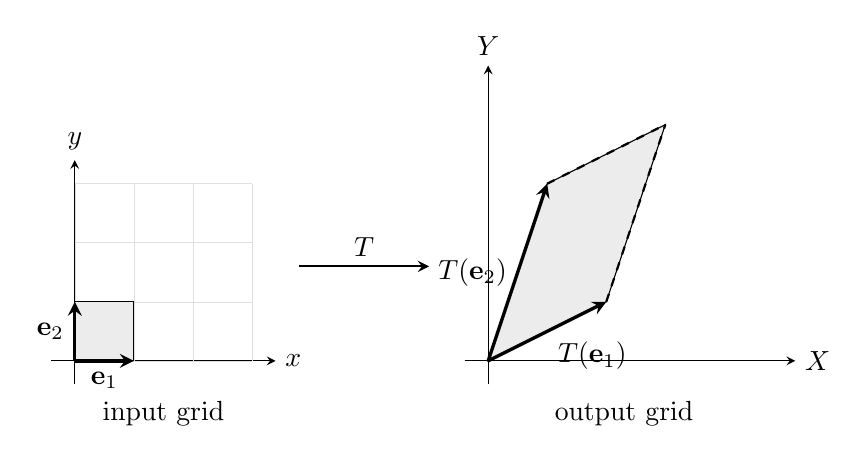
\begin{tikzpicture}[scale=0.75, >=stealth]
    \begin{scope}
        \draw[->] (-0.4,0) -- (3.4,0) node[right] {\(x\)};
        \draw[->] (0,-0.4) -- (0,3.4) node[above] {\(y\)};
        \draw[step=1, gray!25, very thin] (0,0) grid (3,3);

        \draw[fill=gray!15] (0,0) -- (1,0) -- (1,1) -- (0,1) -- cycle;
        \draw[->, very thick] (0,0) -- (1,0) node[midway, below] {\(\mathbf e_1\)};
        \draw[->, very thick] (0,0) -- (0,1) node[midway, left] {\(\mathbf e_2\)};
        \node at (1.5,-0.9) {input grid};
    \end{scope}

    \begin{scope}[shift={(7,0)}]
        \draw[->] (-0.4,0) -- (5.2,0) node[right] {\(X\)};
        \draw[->] (0,-0.4) -- (0,5.0) node[above] {\(Y\)};

        \coordinate (O) at (0,0);
        \coordinate (U) at (2,1);
        \coordinate (V) at (1,3);
        \coordinate (UV) at (3,4);

        \draw[fill=gray!15] (O) -- (U) -- (UV) -- (V) -- cycle;
        \draw[->, very thick] (O) -- (U) node[midway, below right] {\(T(\mathbf e_1)\)};
        \draw[->, very thick] (O) -- (V) node[midway, left] {\(T(\mathbf e_2)\)};
        \draw[thick, dashed] (U) -- (UV);
        \draw[thick, dashed] (V) -- (UV);
        \node at (2.3,-0.9) {output grid};
    \end{scope}

    \draw[->, thick] (3.8,1.6) -- (6.0,1.6) node[midway, above] {\(T\)};
\end{tikzpicture}
\caption{A linear transformation sends the standard unit square to the parallelogram
spanned by the images of \(\mathbf e_1\) and \(\mathbf e_2\).}
\end{figure}

This example contains the main idea.  Once we know where the basic directions go,
linearity tells us where every vector goes.

\begin{definition}[Linear transformation]
A function
\[
    T:\mathbb R^n\to\mathbb R^m
\]
is called a \emph{linear transformation} if, for all vectors
\[
    \mathbf u,\mathbf v\in\mathbb R^n
\]
and all scalars \(c\),
\[
    T(\mathbf u+\mathbf v)=T(\mathbf u)+T(\mathbf v),
\]
and
\[
    T(c\mathbf u)=cT(\mathbf u).
\]
\end{definition}

The definition is the same as the definition of a linear function, except that the output
is now a vector.

A linear transformation must send the zero vector to the zero vector:
\[
    T(\mathbf 0)=\mathbf 0.
\]
So translations are not linear.

\begin{example}[A translation is not linear]
The rule
\[
    F(x,y)=(x+1,y)
\]
moves every point one unit to the right.  It is a perfectly useful geometric motion, but
it is not linear because
\[
    F(0,0)=(1,0)\neq(0,0).
\]
Also,
\[
    F((1,0)+(0,1))=F(1,1)=(2,1),
\]
while
\[
    F(1,0)+F(0,1)=(2,0)+(1,1)=(3,1).
\]
The addition rule fails.
\end{example}

Translations will return when we discuss affine maps and tangent planes.  For now,
linear transformations are the origin-fixing machines.

\subsection{Images of basis vectors determine the whole map}

The grid example was not special.

Let
\[
    T:\mathbb R^n\to\mathbb R^m
\]
be linear.  Every input vector can be written as
\[
    \mathbf x=x_1\mathbf e_1+\cdots+x_n\mathbf e_n.
\]
Then linearity forces
\[
\boxed{
    T(\mathbf x)
    =
    x_1T(\mathbf e_1)+\cdots+x_nT(\mathbf e_n).
}
\]

So the entire transformation is determined by the \(n\) output vectors
\[
    T(\mathbf e_1),\quad T(\mathbf e_2),\quad \ldots,\quad T(\mathbf e_n).
\]

\begin{theorem}[A linear transformation is determined by its values on the standard basis]
Let
\[
    T:\mathbb R^n\to\mathbb R^m
\]
be linear.  Then, for every
\[
    \mathbf x=(x_1,\ldots,x_n),
\]
\[
\boxed{
    T(\mathbf x)
    =
    x_1T(\mathbf e_1)+x_2T(\mathbf e_2)+\cdots+x_nT(\mathbf e_n).
}
\]
\end{theorem}

\begin{proof}
Use the standard basis expansion
\[
    \mathbf x=x_1\mathbf e_1+x_2\mathbf e_2+\cdots+x_n\mathbf e_n.
\]
Then apply linearity:
\[
\begin{aligned}
T(\mathbf x)
&=
T(x_1\mathbf e_1+x_2\mathbf e_2+\cdots+x_n\mathbf e_n)\\
&=
x_1T(\mathbf e_1)+x_2T(\mathbf e_2)+\cdots+x_nT(\mathbf e_n).
\end{aligned}
\]
\end{proof}

The hypothesis that \(T\) is linear is essential.

\begin{example}[Without linearity, basis vectors are not enough]
Consider two maps from \(\mathbb R^2\) to \(\mathbb R^2\):
\[
    I(x,y)=(x,y)
\]
and
\[
    N(x,y)=(x^2,y).
\]
They agree on the standard basis:
\[
    I(1,0)=(1,0)=N(1,0),
\]
and
\[
    I(0,1)=(0,1)=N(0,1).
\]
But they do not agree everywhere:
\[
    I(2,0)=(2,0),
\]
while
\[
    N(2,0)=(4,0).
\]
The map \(N\) is not linear.  Knowing what it does to the basis vectors does not
determine what it does to every vector.
\end{example}

Linearity is what lets the basic directions control the whole map.

\subsection{Matrices as representations of linear transformations}

For the grid machine above,
\[
    T(\mathbf e_1)=(2,1),
    \qquad
    T(\mathbf e_2)=(1,3).
\]
It is convenient to store these two output vectors as the columns of a rectangular array:
\[
    A=
    \begin{pmatrix}
        2&1\\
        1&3
    \end{pmatrix}.
\]
Then
\[
    T(x,y)
    =
    x\begin{pmatrix}2\\1\end{pmatrix}
    +
    y\begin{pmatrix}1\\3\end{pmatrix}
    =
    \begin{pmatrix}
        2x+y\\
        x+3y
    \end{pmatrix}.
\]
This is matrix-vector multiplication.

\begin{definition}[Matrix]
An \(m\times n\) matrix is a rectangular array of numbers with \(m\) rows and \(n\)
columns:
\[
    A=
    \begin{pmatrix}
        a_{11}&a_{12}&\cdots&a_{1n}\\
        a_{21}&a_{22}&\cdots&a_{2n}\\
        \vdots&\vdots&\ddots&\vdots\\
        a_{m1}&a_{m2}&\cdots&a_{mn}
    \end{pmatrix}.
\]
If its columns are
\[
    \mathbf a_1,\mathbf a_2,\ldots,\mathbf a_n\in\mathbb R^m,
\]
then for
\[
    \mathbf x=(x_1,\ldots,x_n)\in\mathbb R^n,
\]
we define
\[
\boxed{
    A\mathbf x
    =
    x_1\mathbf a_1+x_2\mathbf a_2+\cdots+x_n\mathbf a_n.
}
\]
\end{definition}

This definition says that a matrix acts by mixing its columns according to the input
coordinates.

In row form, the same multiplication is
\[
    A\mathbf x
    =
    \begin{pmatrix}
        a_{11}x_1+a_{12}x_2+\cdots+a_{1n}x_n\\
        a_{21}x_1+a_{22}x_2+\cdots+a_{2n}x_n\\
        \vdots\\
        a_{m1}x_1+a_{m2}x_2+\cdots+a_{mn}x_n
    \end{pmatrix}.
\]
Each output coordinate is a linear function of the input.

\begin{example}[A \(2\times 3\) matrix]
Let
\[
    A=
    \begin{pmatrix}
        1&2&0\\
        0&-1&3
    \end{pmatrix}.
\]
Then \(A\) takes inputs from \(\mathbb R^3\) and produces outputs in \(\mathbb R^2\):
\[
    A:\mathbb R^3\to\mathbb R^2.
\]
For
\[
    \mathbf x=(x,y,z),
\]
\[
    A\mathbf x
    =
    \begin{pmatrix}
        x+2y\\
        -y+3z
    \end{pmatrix}.
\]
For example,
\[
    A(4,1,2)
    =
    \begin{pmatrix}
        4+2\\
        -1+6
    \end{pmatrix}
    =
    \begin{pmatrix}
        6\\
        5
    \end{pmatrix}.
\]
\end{example}

Now the relationship between matrices and linear transformations can be stated cleanly.

\begin{theorem}[Every linear transformation has a matrix]
Let
\[
    T:\mathbb R^n\to\mathbb R^m
\]
be linear.  Form the matrix
\[
    A=
    \begin{pmatrix}
        |&|&&|\\
        T(\mathbf e_1)&T(\mathbf e_2)&\cdots&T(\mathbf e_n)\\
        |&|&&|
    \end{pmatrix},
\]
whose columns are the images of the standard basis vectors.  Then
\[
\boxed{
    T(\mathbf x)=A\mathbf x
}
\]
for every \(\mathbf x\in\mathbb R^n\).

Conversely, every \(m\times n\) matrix \(A\) defines a linear transformation
\[
    \mathbf x\longmapsto A\mathbf x
\]
from \(\mathbb R^n\) to \(\mathbb R^m\).
\end{theorem}

\begin{proof}
Let
\[
    \mathbf x=(x_1,\ldots,x_n).
\]
By the previous theorem,
\[
    T(\mathbf x)
    =
    x_1T(\mathbf e_1)+\cdots+x_nT(\mathbf e_n).
\]
But the columns of \(A\) are exactly
\[
    T(\mathbf e_1),\ldots,T(\mathbf e_n).
\]
So the right-hand side is precisely
\[
    A\mathbf x.
\]

Conversely, suppose \(A\) is an \(m\times n\) matrix with columns
\[
    \mathbf a_1,\ldots,\mathbf a_n.
\]
For vectors
\[
    \mathbf x=(x_1,\ldots,x_n),
    \qquad
    \mathbf y=(y_1,\ldots,y_n),
\]
we have
\[
\begin{aligned}
A(\mathbf x+\mathbf y)
&=
A(x_1+y_1,\ldots,x_n+y_n)\\
&=
(x_1+y_1)\mathbf a_1+\cdots+(x_n+y_n)\mathbf a_n\\
&=
(x_1\mathbf a_1+\cdots+x_n\mathbf a_n)
+
(y_1\mathbf a_1+\cdots+y_n\mathbf a_n)\\
&=
A\mathbf x+A\mathbf y.
\end{aligned}
\]
Also,
\[
    A(c\mathbf x)=cA\mathbf x.
\]
So the map \(\mathbf x\mapsto A\mathbf x\) is linear.
\end{proof}

A matrix is the coordinate record of a linear transformation.  It is not the geometric
machine itself; it is the machine written in a chosen coordinate language.

\subsection{Rows, columns, inputs, and outputs}

The columns tell us where the basis vectors go.

For
\[
    A=
    \begin{pmatrix}
        2&1\\
        1&3
    \end{pmatrix},
\]
the first column says
\[
    A\mathbf e_1=(2,1),
\]
and the second column says
\[
    A\mathbf e_2=(1,3).
\]

The rows tell us the output measurements.

The first row
\[
    (2,1)
\]
produces the first coordinate:
\[
    2x+y.
\]
The second row
\[
    (1,3)
\]
produces the second coordinate:
\[
    x+3y.
\]
So a matrix has two equally important readings:
\[
\begin{array}{c|c}
\text{Columns} & \text{images of input basis vectors}\\ \hline
\text{Rows} & \text{linear functions giving output coordinates}
\end{array}
\]

The size of a matrix follows the direction of the transformation:
\[
    T:\mathbb R^n\to\mathbb R^m
    \qquad\Longleftrightarrow\qquad
    A\text{ is }m\times n.
\]
The input dimension \(n\) is the number of columns.  The output dimension \(m\) is the
number of rows.

\[
\begin{array}{c|c|c}
\text{Transformation} & \text{Matrix size} & \text{Example} \\ \hline
\mathbb R^2\to\mathbb R^2 & 2\times2
&
\begin{pmatrix}2&1\\1&3\end{pmatrix}
\\[1.2em]
\mathbb R^3\to\mathbb R^2 & 2\times3
&
\begin{pmatrix}1&2&0\\0&-1&3\end{pmatrix}
\\[1.2em]
\mathbb R^2\to\mathbb R^3 & 3\times2
&
\begin{pmatrix}1&0\\0&1\\2&-1\end{pmatrix}
\end{array}
\]

\begin{example}[A projection]
The map
\[
    P:\mathbb R^3\to\mathbb R^2
\]
that drops the height coordinate is
\[
    P(x,y,z)=(x,y).
\]
It is linear.  Its matrix is
\[
    P=
    \begin{pmatrix}
        1&0&0\\
        0&1&0
    \end{pmatrix}.
\]
The columns tell us
\[
    P(\mathbf e_1)=(1,0),
    \qquad
    P(\mathbf e_2)=(0,1),
    \qquad
    P(\mathbf e_3)=(0,0).
\]
The third basis direction is collapsed because vertical motion has no shadow on the
floor.
\end{example}

\begin{example}[A map from the plane into space]
Let
\[
    S:\mathbb R^2\to\mathbb R^3
\]
be defined by
\[
    S(x,y)=(x,\;y,\;2x-y).
\]
This map places the \(xy\)-plane onto the tilted plane
\[
    z=2x-y.
\]
Its matrix is
\[
    A=
    \begin{pmatrix}
        1&0\\
        0&1\\
        2&-1
    \end{pmatrix}.
\]
The columns are
\[
    S(\mathbf e_1)=(1,0,2),
    \qquad
    S(\mathbf e_2)=(0,1,-1).
\]
So the two ordinary coordinate directions in the input plane become two direction
vectors lying in the tilted plane.
\end{example}

This is the first time matrices have appeared as objects of their own.  But their real
power shows up when machines are connected.  If one linear transformation moves a
grid and a second transformation moves the new grid again, the combined effect is
still linear.  The question is not whether it has a matrix.  It does.  The question is how
to compute that matrix without rebuilding the whole machine from scratch.  That
question forces the rule for multiplying matrices.
%% --- 3.3  [Core] ---
\section{Matrix multiplication as composition}
\label{sec:3.3}

Section 3.2 ended with a linear transformation as a machine written in coordinates.
The columns of its matrix tell us where the basic input directions go.  But machines are
rarely used alone.  A camera may first rotate a picture and then crop it.  A robot arm may
first stretch a coordinate grid and then project it onto a screen.  Once two linear machines
are connected, we need a matrix for the combined machine.

That need is the real reason matrix multiplication exists.

\subsection{Applying one linear map after another}

Start with the linear transformation
\[
    A:\mathbb R^2\to\mathbb R^2
\]
given by
\[
    A(x,y)=
    \begin{pmatrix}
        2&1\\
        1&3
    \end{pmatrix}
    \begin{pmatrix}x\\y\end{pmatrix}
    =
    \begin{pmatrix}
        2x+y\\
        x+3y
    \end{pmatrix}.
\]
This machine stretches and shears the grid.  Now send the result through a second
machine
\[
    B:\mathbb R^2\to\mathbb R^2,
    \qquad
    B(X,Y)=
    \begin{pmatrix}
        1&0\\
        2&1
    \end{pmatrix}
    \begin{pmatrix}X\\Y\end{pmatrix}
    =
    \begin{pmatrix}
        X\\
        2X+Y
    \end{pmatrix}.
\]
The capital letters \(X,Y\) remind us that \(B\) acts on the output of \(A\).

Let us follow one point:
\[
    \mathbf x=(4,2).
\]
First apply \(A\):
\[
    A(4,2)
    =
    \begin{pmatrix}
        2\cdot4+2\\
        4+3\cdot2
    \end{pmatrix}
    =
    \begin{pmatrix}
        10\\
        10
    \end{pmatrix}.
\]
Then apply \(B\):
\[
    B(A(4,2))
    =
    B(10,10)
    =
    \begin{pmatrix}
        10\\
        2\cdot10+10
    \end{pmatrix}
    =
    \begin{pmatrix}
        10\\
        30
    \end{pmatrix}.
\]

We can also compute the combined rule directly.  Since
\[
    A(x,y)=(2x+y,\;x+3y),
\]
we get
\[
\begin{aligned}
    B(A(x,y))
    &=
    B(2x+y,\;x+3y)\\
    &=
    \bigl(2x+y,\;2(2x+y)+(x+3y)\bigr)\\
    &=
    (2x+y,\;5x+5y).
\end{aligned}
\]
So the combined machine is
\[
    (x,y)\longmapsto (2x+y,\;5x+5y).
\]
Its matrix is
\[
    \begin{pmatrix}
        2&1\\
        5&5
    \end{pmatrix}.
\]

This matrix is not guessed.  It comes from the columns.  The first column is the image
of \(\mathbf e_1\) after both machines:
\[
    A\mathbf e_1=
    \begin{pmatrix}2\\1\end{pmatrix},
    \qquad
    B(A\mathbf e_1)=
    B\begin{pmatrix}2\\1\end{pmatrix}
    =
    \begin{pmatrix}2\\5\end{pmatrix}.
\]
The second column is the image of \(\mathbf e_2\) after both machines:
\[
    A\mathbf e_2=
    \begin{pmatrix}1\\3\end{pmatrix},
    \qquad
    B(A\mathbf e_2)=
    B\begin{pmatrix}1\\3\end{pmatrix}
    =
    \begin{pmatrix}1\\5\end{pmatrix}.
\]
Therefore the matrix of the combined transformation is
\[
    \begin{pmatrix}
        2&1\\
        5&5
    \end{pmatrix}.
\]

\begin{definition}[Composition]
If
\[
    S:\mathbb R^n\to\mathbb R^m
\]
and
\[
    T:\mathbb R^m\to\mathbb R^p,
\]
then the \emph{composition}
\[
    T\circ S:\mathbb R^n\to\mathbb R^p
\]
is the function
\[
    (T\circ S)(\mathbf x)=T(S(\mathbf x)).
\]
The map \(S\) acts first, and \(T\) acts second.
\end{definition}

The notation is read from right to left:
\[
    T\circ S
    \qquad
    \text{means}
    \qquad
    \text{first }S,\text{ then }T.
\]

\begin{theorem}[A composition of linear transformations is linear]
Let
\[
    S:\mathbb R^n\to\mathbb R^m
\]
and
\[
    T:\mathbb R^m\to\mathbb R^p
\]
be linear transformations.  Then
\[
    T\circ S:\mathbb R^n\to\mathbb R^p
\]
is linear.
\end{theorem}

\begin{proof}
For vectors \(\mathbf u,\mathbf v\in\mathbb R^n\),
\[
\begin{aligned}
(T\circ S)(\mathbf u+\mathbf v)
&=
T(S(\mathbf u+\mathbf v))\\
&=
T(S(\mathbf u)+S(\mathbf v))\\
&=
T(S(\mathbf u))+T(S(\mathbf v))\\
&=
(T\circ S)(\mathbf u)+(T\circ S)(\mathbf v).
\end{aligned}
\]
Also, for a scalar \(c\),
\[
\begin{aligned}
(T\circ S)(c\mathbf u)
&=
T(S(c\mathbf u))\\
&=
T(cS(\mathbf u))\\
&=
cT(S(\mathbf u))\\
&=
c(T\circ S)(\mathbf u).
\end{aligned}
\]
So \(T\circ S\) respects addition and scaling.
\end{proof}

The hypotheses are doing real work.  If the first map is not linear, the composition need
not be linear.

\begin{example}[A nonlinear first step breaks linearity]
Let
\[
    S(x,y)=(x^2,y)
\]
and let
\[
    T(X,Y)=(X+Y,Y).
\]
The second map \(T\) is linear, but \(S\) is not.  The composition is
\[
    (T\circ S)(x,y)=T(x^2,y)=(x^2+y,y).
\]
This is not linear because
\[
    (T\circ S)(2,0)=(4,0),
\]
but
\[
    2(T\circ S)(1,0)=2(1,0)=(2,0).
\]
A single nonlinear step can bend the whole machine.
\end{example}

\subsection{The matrix of a composition}

The example above gives the rule.

Let \(A\) be an \(m\times n\) matrix.  It represents a linear transformation
\[
    A:\mathbb R^n\to\mathbb R^m.
\]
Let \(B\) be a \(p\times m\) matrix.  It represents a linear transformation
\[
    B:\mathbb R^m\to\mathbb R^p.
\]
Then the combined transformation is
\[
    \mathbf x\longmapsto B(A\mathbf x).
\]
Its matrix is called
\[
    BA.
\]

The columns of \(BA\) are easy to describe.  If the columns of \(A\) are
\[
    \mathbf a_1,\mathbf a_2,\ldots,\mathbf a_n,
\]
then
\[
    A\mathbf e_j=\mathbf a_j.
\]
After applying \(B\),
\[
    B(A\mathbf e_j)=B\mathbf a_j.
\]
So the \(j\)-th column of \(BA\) is
\[
    B\mathbf a_j.
\]

\begin{definition}[Matrix multiplication]
Let \(A\) be an \(m\times n\) matrix with columns
\[
    \mathbf a_1,\ldots,\mathbf a_n\in\mathbb R^m,
\]
and let \(B\) be a \(p\times m\) matrix.  The product
\[
    BA
\]
is the \(p\times n\) matrix whose columns are
\[
    B\mathbf a_1,\;B\mathbf a_2,\;\ldots,\;B\mathbf a_n.
\]
Equivalently,
\[
\boxed{
    BA=
    \begin{pmatrix}
        |&|&&|\\
        B\mathbf a_1&B\mathbf a_2&\cdots&B\mathbf a_n\\
        |&|&&|
    \end{pmatrix}.
}
\]
\end{definition}

This is the cleanest meaning of matrix multiplication:

\[
\boxed{
    \text{matrix multiplication records composition of linear transformations.}
}
\]

\begin{example}[Multiplying two matrices by columns]
Let
\[
    A=
    \begin{pmatrix}
        2&1\\
        1&3
    \end{pmatrix},
    \qquad
    B=
    \begin{pmatrix}
        1&0\\
        2&1
    \end{pmatrix}.
\]
The columns of \(A\) are
\[
    \mathbf a_1=
    \begin{pmatrix}2\\1\end{pmatrix},
    \qquad
    \mathbf a_2=
    \begin{pmatrix}1\\3\end{pmatrix}.
\]
Apply \(B\) to each:
\[
    B\mathbf a_1
    =
    \begin{pmatrix}
        1&0\\
        2&1
    \end{pmatrix}
    \begin{pmatrix}2\\1\end{pmatrix}
    =
    \begin{pmatrix}2\\5\end{pmatrix},
\]
and
\[
    B\mathbf a_2
    =
    \begin{pmatrix}
        1&0\\
        2&1
    \end{pmatrix}
    \begin{pmatrix}1\\3\end{pmatrix}
    =
    \begin{pmatrix}1\\5\end{pmatrix}.
\]
Therefore
\[
    BA=
    \begin{pmatrix}
        2&1\\
        5&5
    \end{pmatrix}.
\]
\end{example}

There is also a row-by-column formula.  If
\[
    A=(a_{ij})
\]
is \(m\times n\), and
\[
    B=(b_{ij})
\]
is \(p\times m\), then \(BA\) is \(p\times n\), and its \((i,j)\)-entry is
\[
\boxed{
    (BA)_{ij}
    =
    b_{i1}a_{1j}+b_{i2}a_{2j}+\cdots+b_{im}a_{mj}.
}
\]
This formula is useful for calculation, but the meaning is the same: first apply \(A\),
then apply \(B\).

\subsection{Why matrix multiplication is ordered}

The order matters because the machines are connected in order.

Using the same two matrices,
\[
    A=
    \begin{pmatrix}
        2&1\\
        1&3
    \end{pmatrix},
    \qquad
    B=
    \begin{pmatrix}
        1&0\\
        2&1
    \end{pmatrix},
\]
we found
\[
    BA=
    \begin{pmatrix}
        2&1\\
        5&5
    \end{pmatrix}.
\]

Now reverse the order.  Compute \(AB\).  The columns of \(B\) are
\[
    \begin{pmatrix}1\\2\end{pmatrix},
    \qquad
    \begin{pmatrix}0\\1\end{pmatrix}.
\]
Applying \(A\) to them gives
\[
    A\begin{pmatrix}1\\2\end{pmatrix}
    =
    \begin{pmatrix}4\\7\end{pmatrix},
    \qquad
    A\begin{pmatrix}0\\1\end{pmatrix}
    =
    \begin{pmatrix}1\\3\end{pmatrix}.
\]
So
\[
    AB=
    \begin{pmatrix}
        4&1\\
        7&3
    \end{pmatrix}.
\]
Thus
\[
    AB\neq BA.
\]

\begin{example}[Two simple moves in different orders]
Let
\[
    R=
    \begin{pmatrix}
        0&-1\\
        1&0
    \end{pmatrix}
\]
be a \(90^\circ\) counterclockwise rotation, and let
\[
    P=
    \begin{pmatrix}
        1&0\\
        0&0
    \end{pmatrix}
\]
be projection onto the \(x\)-axis.

Apply them to
\[
    \mathbf x=(1,2).
\]

First rotate, then project:
\[
    R(1,2)=(-2,1),
    \qquad
    P(R(1,2))=(-2,0).
\]

First project, then rotate:
\[
    P(1,2)=(1,0),
    \qquad
    R(P(1,2))=(0,1).
\]

The answers are different:
\[
    PR(1,2)=(-2,0),
    \qquad
    RP(1,2)=(0,1).
\]
Projection throws away information.  Whether we throw it away before or after rotating
changes the result.
\end{example}

\begin{figure}[h]
\centering
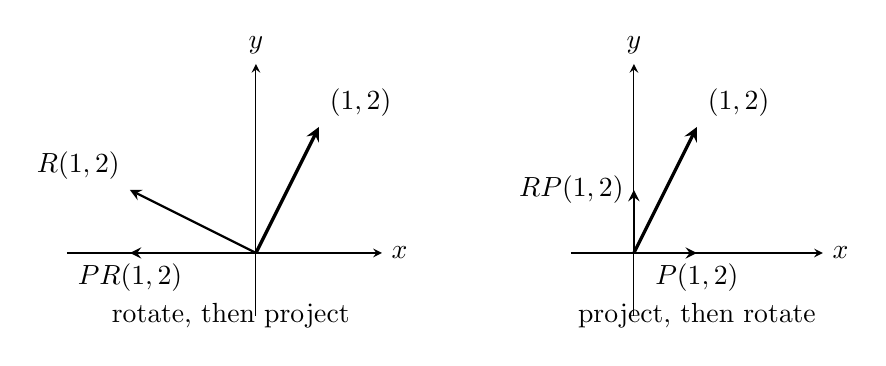
\begin{tikzpicture}[scale=0.8, >=stealth]
    \begin{scope}
        \draw[->] (-3,0) -- (2,0) node[right] {\(x\)};
        \draw[->] (0,-1) -- (0,3) node[above] {\(y\)};
        \draw[->, very thick] (0,0) -- (1,2) node[above right] {\((1,2)\)};
        \draw[->, thick] (0,0) -- (-2,1) node[above left] {\(R(1,2)\)};
        \draw[->, thick] (0,0) -- (-2,0) node[below] {\(PR(1,2)\)};
        \node at (-0.4,-1.0) {rotate, then project};
    \end{scope}

    \begin{scope}[shift={(6,0)}]
        \draw[->] (-1,0) -- (3,0) node[right] {\(x\)};
        \draw[->] (0,-1) -- (0,3) node[above] {\(y\)};
        \draw[->, very thick] (0,0) -- (1,2) node[above right] {\((1,2)\)};
        \draw[->, thick] (0,0) -- (1,0) node[below] {\(P(1,2)\)};
        \draw[->, thick] (0,0) -- (0,1) node[left] {\(RP(1,2)\)};
        \node at (1.0,-1.0) {project, then rotate};
    \end{scope}
\end{tikzpicture}
\caption{Changing the order of two linear transformations can change the result.}
\end{figure}

Matrix multiplication is usually not commutative:
\[
    AB\neq BA.
\]
This is not a flaw in the notation.  It is the notation telling the truth.

\subsection{Identity matrices and inverse matrices}

Some machines do nothing.  In \(\mathbb R^2\), the matrix
\[
    I_2=
    \begin{pmatrix}
        1&0\\
        0&1
    \end{pmatrix}
\]
satisfies
\[
    I_2
    \begin{pmatrix}x\\y\end{pmatrix}
    =
    \begin{pmatrix}x\\y\end{pmatrix}.
\]
In \(\mathbb R^3\),
\[
    I_3=
    \begin{pmatrix}
        1&0&0\\
        0&1&0\\
        0&0&1
    \end{pmatrix}.
\]

\begin{definition}[Identity matrix]
The \(n\times n\) identity matrix is
\[
    I_n=
    \begin{pmatrix}
        1&0&\cdots&0\\
        0&1&\cdots&0\\
        \vdots&\vdots&\ddots&\vdots\\
        0&0&\cdots&1
    \end{pmatrix}.
\]
It satisfies
\[
    I_n\mathbf x=\mathbf x
\]
for every \(\mathbf x\in\mathbb R^n\).
\end{definition}

If \(A\) is \(m\times n\), then
\[
    AI_n=A,
    \qquad
    I_mA=A.
\]
The identity matrix is the matrix version of multiplying by \(1\).

Some machines can be undone.  If a matrix \(A\) transforms the grid without collapsing
information, there may be another matrix that reverses its effect.

\begin{definition}[Inverse matrix]
Let \(A\) be an \(n\times n\) matrix.  An \(n\times n\) matrix \(A^{-1}\) is called the
\emph{inverse} of \(A\) if
\[
    A^{-1}A=I_n
    \qquad\text{and}\qquad
    AA^{-1}=I_n.
\]
If such a matrix exists, \(A\) is called \emph{invertible}.
\end{definition}

\begin{example}[Undoing a linear transformation]
Let
\[
    A=
    \begin{pmatrix}
        2&1\\
        1&1
    \end{pmatrix}
\]
and
\[
    C=
    \begin{pmatrix}
        1&-1\\
        -1&2
    \end{pmatrix}.
\]
Then
\[
    CA=
    \begin{pmatrix}
        1&-1\\
        -1&2
    \end{pmatrix}
    \begin{pmatrix}
        2&1\\
        1&1
    \end{pmatrix}
    =
    \begin{pmatrix}
        1&0\\
        0&1
    \end{pmatrix}.
\]
Also,
\[
    AC=
    \begin{pmatrix}
        2&1\\
        1&1
    \end{pmatrix}
    \begin{pmatrix}
        1&-1\\
        -1&2
    \end{pmatrix}
    =
    \begin{pmatrix}
        1&0\\
        0&1
    \end{pmatrix}.
\]
So
\[
    C=A^{-1}.
\]

For instance,
\[
    A(3,1)=(7,4).
\]
Applying the inverse gives
\[
    A^{-1}(7,4)
    =
    \begin{pmatrix}
        1&-1\\
        -1&2
    \end{pmatrix}
    \begin{pmatrix}7\\4\end{pmatrix}
    =
    \begin{pmatrix}3\\1\end{pmatrix}.
\]
The inverse recovers the original input.
\end{example}

The requirement that \(A\) be square is important for a two-sided inverse.

\begin{example}[Why not every useful map has an inverse]
The projection
\[
    P:\mathbb R^3\to\mathbb R^2,
    \qquad
    P(x,y,z)=(x,y),
\]
has matrix
\[
    P=
    \begin{pmatrix}
        1&0&0\\
        0&1&0
    \end{pmatrix}.
\]
It loses the height coordinate.  For example,
\[
    P(2,5,0)=(2,5),
\]
and
\[
    P(2,5,100)=(2,5).
\]
No function can recover the original height from the output alone.

The inclusion
\[
    S:\mathbb R^2\to\mathbb R^3,
    \qquad
    S(x,y)=(x,y,0),
\]
has the opposite problem.  It does not lose information from the input, but it only reaches
the plane \(z=0\).  No inverse from all of \(\mathbb R^3\) back to \(\mathbb R^2\) can undo
it everywhere.

A true two-sided inverse is a square-machine idea: same input dimension, same output
dimension, no information lost, and nothing unreachable.
\end{example}

\subsection{Rotations, reflections, projections, and shears}

Many familiar geometric moves are linear transformations.

\[
\begin{array}{c|c|c}
\text{Transformation} & \text{Matrix} & \text{Effect on }(x,y) \\ \hline
\text{rotation by }\theta
&
\begin{pmatrix}
\cos\theta&-\sin\theta\\
\sin\theta&\cos\theta
\end{pmatrix}
&
(x\cos\theta-y\sin\theta,\;x\sin\theta+y\cos\theta)
\\[1.4em]
\text{reflection across the }x\text{-axis}
&
\begin{pmatrix}
1&0\\
0&-1
\end{pmatrix}
&
(x,-y)
\\[1.4em]
\text{projection onto the }x\text{-axis}
&
\begin{pmatrix}
1&0\\
0&0
\end{pmatrix}
&
(x,0)
\\[1.4em]
\text{horizontal shear}
&
\begin{pmatrix}
1&k\\
0&1
\end{pmatrix}
&
(x+ky,y)
\end{array}
\]

The columns still tell the story.

For a rotation by \(\theta\),
\[
    \mathbf e_1\longmapsto(\cos\theta,\sin\theta),
\]
and
\[
    \mathbf e_2\longmapsto(-\sin\theta,\cos\theta).
\]
These are the two rotated coordinate directions.

For a projection onto the \(x\)-axis,
\[
    \mathbf e_1\longmapsto \mathbf e_1,
    \qquad
    \mathbf e_2\longmapsto \mathbf 0.
\]
The vertical direction is collapsed.

For a shear,
\[
    \mathbf e_1\longmapsto \mathbf e_1,
    \qquad
    \mathbf e_2\longmapsto(k,1).
\]
Vertical lines tilt, but horizontal lines stay horizontal.

\begin{example}[Composing rotations]
Let \(R_\alpha\) be rotation by angle \(\alpha\), and let \(R_\beta\) be rotation by angle
\(\beta\).  Rotating first by \(\alpha\) and then by \(\beta\) should be the same as rotating
by \(\alpha+\beta\):
\[
    R_\beta R_\alpha=R_{\alpha+\beta}.
\]
Matrix multiplication turns this geometric fact into the angle-addition formulas:
\[
\begin{pmatrix}
\cos\beta&-\sin\beta\\
\sin\beta&\cos\beta
\end{pmatrix}
\begin{pmatrix}
\cos\alpha&-\sin\alpha\\
\sin\alpha&\cos\alpha
\end{pmatrix}
=
\begin{pmatrix}
\cos(\alpha+\beta)&-\sin(\alpha+\beta)\\
\sin(\alpha+\beta)&\cos(\alpha+\beta)
\end{pmatrix}.
\]
Here a familiar trigonometric identity is really a statement about composing two
linear transformations.
\end{example}

Matrix multiplication lets us keep track of connected machines.  But it does not yet tell
us everything we want to know about those machines.  A rotation turns a square without
changing its area.  A shear slants it without changing area.  A projection flattens it to a
line and destroys its area completely.  Somewhere inside a square matrix there must be a
single number that measures this area or volume effect.  Chapter 2 already gave that
number a name: the determinant.

\section{Determinants of linear transformations}
\label{sec:3.4}

Chapter 2 introduced determinants as signed area in the plane and signed volume in
space.  Section 3.3 showed that a matrix is a linear machine.  Now these two ideas meet:
the determinant of a square matrix tells us how that machine changes area or volume.

\subsection{Area scaling under a matrix}

Return to the matrix from the grid example:
\[
    A=
    \begin{pmatrix}
        2&1\\
        1&3
    \end{pmatrix}.
\]
Its columns are
\[
    \mathbf a_1=(2,1),
    \qquad
    \mathbf a_2=(1,3).
\]
The standard unit square is spanned by
\[
    \mathbf e_1=(1,0),
    \qquad
    \mathbf e_2=(0,1).
\]
The matrix \(A\) sends that square to the parallelogram spanned by
\[
    A\mathbf e_1=\mathbf a_1=(2,1),
    \qquad
    A\mathbf e_2=\mathbf a_2=(1,3).
\]

The signed area of this parallelogram is
\[
    \det
    \begin{pmatrix}
        2&1\\
        1&3
    \end{pmatrix}
    =
    2\cdot3-1\cdot1
    =
    5.
\]
So \(A\) sends a unit square of area \(1\) to a parallelogram of area \(5\).

\begin{figure}[h]
\centering
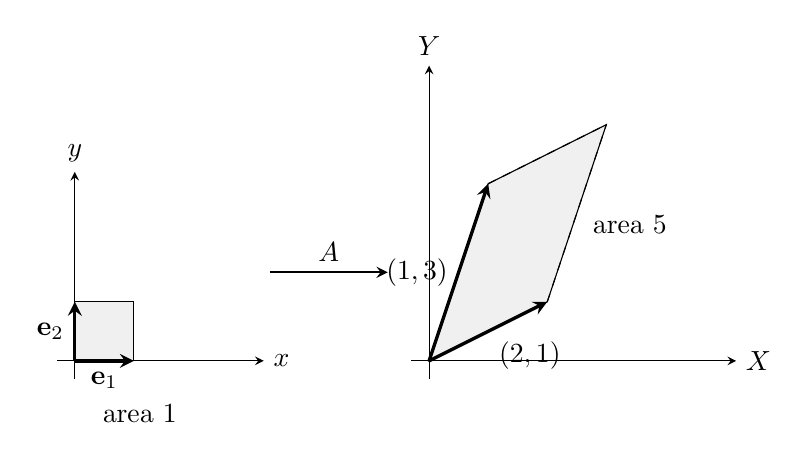
\begin{tikzpicture}[scale=0.75, >=stealth]
    \begin{scope}
        \draw[->] (-0.3,0) -- (3.2,0) node[right] {\(x\)};
        \draw[->] (0,-0.3) -- (0,3.2) node[above] {\(y\)};
        \draw[fill=gray!12] (0,0) -- (1,0) -- (1,1) -- (0,1) -- cycle;
        \draw[->, very thick] (0,0) -- (1,0) node[midway, below] {\(\mathbf e_1\)};
        \draw[->, very thick] (0,0) -- (0,1) node[midway, left] {\(\mathbf e_2\)};
        \node at (1.1,-0.9) {area \(1\)};
    \end{scope}

    \begin{scope}[shift={(6,0)}]
        \draw[->] (-0.3,0) -- (5.2,0) node[right] {\(X\)};
        \draw[->] (0,-0.3) -- (0,5.0) node[above] {\(Y\)};

        \coordinate (O) at (0,0);
        \coordinate (A1) at (2,1);
        \coordinate (A2) at (1,3);
        \coordinate (S) at (3,4);

        \draw[fill=gray!12] (O) -- (A1) -- (S) -- (A2) -- cycle;
        \draw[->, very thick] (O) -- (A1) node[midway, below right] {\((2,1)\)};
        \draw[->, very thick] (O) -- (A2) node[midway, left] {\((1,3)\)};
        \draw[dashed] (A1) -- (S);
        \draw[dashed] (A2) -- (S);
        \node at (3.4,2.3) {area \(5\)};
    \end{scope}

    \draw[->, thick] (3.3,1.5) -- (5.3,1.5) node[midway, above] {\(A\)};
\end{tikzpicture}
\caption{The unit square maps to the parallelogram spanned by the columns of \(A\).}
\end{figure}

This example already contains the general rule.

\begin{definition}[Determinant of a \(2\times2\) matrix]
For
\[
    A=
    \begin{pmatrix}
        a&b\\
        c&d
    \end{pmatrix},
\]
the determinant of \(A\) is
\[
\boxed{
    \det A=ad-bc.
}
\]
Equivalently, if the columns of \(A\) are
\[
    \mathbf a_1=(a,c),
    \qquad
    \mathbf a_2=(b,d),
\]
then \(\det A\) is the signed area of the parallelogram spanned by
\[
    \mathbf a_1,\mathbf a_2.
\]
\end{definition}

\begin{theorem}[Area scaling in the plane]
Let \(A\) be a \(2\times2\) matrix.  If \(P\) is a parallelogram in the plane, then
\[
\boxed{
    \text{signed area of }A(P)
    =
    (\det A)(\text{signed area of }P).
}
\]
For ordinary, unsigned area,
\[
\boxed{
    \text{area of }A(P)
    =
    |\det A|\,\text{area of }P.
}
\]
\end{theorem}

\begin{proof}
Suppose \(P\) is spanned by the vectors
\[
    \mathbf u=(u_1,u_2),
    \qquad
    \mathbf v=(v_1,v_2).
\]
Its signed area is
\[
    \det
    \begin{pmatrix}
        u_1&v_1\\
        u_2&v_2
    \end{pmatrix}.
\]
The image \(A(P)\) is spanned by
\[
    A\mathbf u,
    \qquad
    A\mathbf v.
\]
A direct expansion shows that
\[
    \det
    \begin{pmatrix}
        |&|\\
        A\mathbf u&A\mathbf v\\
        |&|
    \end{pmatrix}
    =
    (\det A)
    \det
    \begin{pmatrix}
        |&|\\
        \mathbf u&\mathbf v\\
        |&|
    \end{pmatrix}.
\]
So the signed area is multiplied by \(\det A\).  Taking absolute values gives the
ordinary area statement.
\end{proof}

The word \emph{linear} is essential.  A nonlinear map may stretch different parts of a
region by different amounts, so no single number can describe its area effect everywhere.

\begin{example}[Why linearity matters]
Consider
\[
    F(x,y)=(x^2,y).
\]
This map is not linear.  It sends the unit square
\[
    0\le x\le1,\qquad 0\le y\le1
\]
onto the same unit square, so the total area stays \(1\).

But the left half of the square,
\[
    0\le x\le \frac12,\qquad 0\le y\le1,
\]
has area
\[
    \frac12.
\]
Its image is
\[
    0\le X\le \frac14,\qquad 0\le Y\le1,
\]
which has area
\[
    \frac14.
\]
So the left half is scaled by a factor of \(\frac12\), while the whole square is scaled
by a factor of \(1\).

There is no single constant area-scaling factor for this nonlinear map.  Later, the
Jacobian determinant will measure the local scaling of such maps, one tiny piece at a
time.
\end{example}

\subsection{Orientation-preserving and orientation-reversing maps}

The determinant has a sign because signed area has a sign.

The ordered pair
\[
    (\mathbf e_1,\mathbf e_2)
\]
is the standard positive orientation of the plane.  If a matrix sends this ordered pair to
two new vectors whose signed area is positive, the matrix preserves orientation.  If the
signed area is negative, it reverses orientation.

\begin{definition}[Orientation in the plane]
A \(2\times2\) matrix \(A\) is called \emph{orientation-preserving} if
\[
    \det A>0.
\]
It is called \emph{orientation-reversing} if
\[
    \det A<0.
\]
If
\[
    \det A=0,
\]
the matrix collapses area and has no genuine two-dimensional orientation.
\end{definition}

\begin{example}[Rotation preserves orientation]
A rotation by \(\theta\) has matrix
\[
    R_\theta=
    \begin{pmatrix}
        \cos\theta&-\sin\theta\\
        \sin\theta&\cos\theta
    \end{pmatrix}.
\]
Its determinant is
\[
\begin{aligned}
    \det R_\theta
    &=
    \cos^2\theta-(-\sin\theta)(\sin\theta)\\
    &=
    \cos^2\theta+\sin^2\theta\\
    &=
    1.
\end{aligned}
\]
A rotation changes direction, but it does not change area or orientation.
\end{example}

\begin{example}[Reflection reverses orientation]
Reflection across the \(x\)-axis has matrix
\[
    H=
    \begin{pmatrix}
        1&0\\
        0&-1
    \end{pmatrix}.
\]
Its determinant is
\[
    \det H=-1.
\]
So it preserves ordinary area but reverses orientation.

Geometrically, the ordered pair
\[
    (\mathbf e_1,\mathbf e_2)
\]
becomes
\[
    (\mathbf e_1,-\mathbf e_2).
\]
The parallelogram has the same size, but its orientation has flipped.
\end{example}

This is exactly the sign behavior of the wedge product from Chapter 2:
\[
    dx\wedge dy=-dy\wedge dx.
\]
Swapping the two directions reverses orientation, and the determinant remembers that
reversal.

\subsection{Singular matrices and collapsed area}

A determinant can also be zero.  That means the matrix collapses two-dimensional area.

\begin{example}[Projection collapses area]
The projection onto the \(x\)-axis is
\[
    P=
    \begin{pmatrix}
        1&0\\
        0&0
    \end{pmatrix}.
\]
It sends
\[
    (x,y)\longmapsto (x,0).
\]
The unit square becomes a line segment:
\[
    0\le x\le1,\qquad y=0.
\]
Its area is \(0\).  The determinant confirms this:
\[
    \det P=1\cdot0-0\cdot0=0.
\]
\end{example}

\begin{example}[Two columns in the same direction]
Let
\[
    A=
    \begin{pmatrix}
        1&2\\
        3&6
    \end{pmatrix}.
\]
The columns are
\[
    \mathbf a_1=(1,3),
    \qquad
    \mathbf a_2=(2,6)=2(1,3).
\]
They point in the same direction.  The unit square maps to a degenerate parallelogram,
which is really just a line segment.

The determinant is
\[
    \det A=1\cdot6-2\cdot3=0.
\]
\end{example}

\begin{theorem}[Zero determinant and collapse in the plane]
For a \(2\times2\) matrix \(A\), the following statements are equivalent:
\[
\begin{array}{ll}
1. & \det A=0,\\
2. & \text{the columns of }A\text{ are linearly dependent},\\
3. & A\text{ collapses the plane onto a line or a point},\\
4. & A\text{ is not invertible}.
\end{array}
\]
\end{theorem}

\begin{proof}
The determinant of \(A\) is the signed area of the parallelogram spanned by its columns.
That area is zero exactly when the two columns lie on one line, which means they are
linearly dependent.

If the columns lie on one line, then every output
\[
    A(x,y)=x(\text{first column})+y(\text{second column})
\]
lies on that same line.  So the plane collapses onto a line, or onto a point if both columns
are zero.

A collapse cannot be inverted, because many different input vectors land on the same
output.  Conversely, if the columns are independent, they form a basis of the plane, so
every output has exactly one coordinate description in those columns.  Then \(A\) is
invertible.
\end{proof}

This theorem is the geometric reason the determinant tests invertibility.  A matrix can
be undone exactly when it has not flattened the plane.

\subsection{Volume scaling in space}

In \(\mathbb R^3\), the determinant measures signed volume.

Let
\[
    A=
    \begin{pmatrix}
        2&0&0\\
        0&3&0\\
        0&0&4
    \end{pmatrix}.
\]
Then
\[
    A(x,y,z)=(2x,3y,4z).
\]
The unit cube becomes a rectangular box with side lengths
\[
    2,\qquad 3,\qquad 4.
\]
Its volume is
\[
    2\cdot3\cdot4=24.
\]
So this matrix multiplies volume by \(24\).

The determinant gives the same number:
\[
    \det A=24.
\]

For a general \(3\times3\) matrix, the determinant is the signed volume of the
parallelepiped spanned by its columns.

\begin{definition}[Determinant of a \(3\times3\) matrix]
Let \(A\) be a \(3\times3\) matrix with columns
\[
    \mathbf a_1,\mathbf a_2,\mathbf a_3.
\]
The determinant of \(A\) is
\[
\boxed{
    \det A=\mathbf a_1\cdot(\mathbf a_2\times\mathbf a_3).
}
\]
Equivalently, if
\[
    A=
    \begin{pmatrix}
        a_{11}&a_{12}&a_{13}\\
        a_{21}&a_{22}&a_{23}\\
        a_{31}&a_{32}&a_{33}
    \end{pmatrix},
\]
then
\[
\boxed{
\begin{aligned}
\det A
&=
a_{11}(a_{22}a_{33}-a_{23}a_{32})\\
&\quad
-a_{12}(a_{21}a_{33}-a_{23}a_{31})\\
&\quad
+a_{13}(a_{21}a_{32}-a_{22}a_{31}).
\end{aligned}
}
\]
\end{definition}

\begin{theorem}[Volume scaling in space]
Let \(A\) be a \(3\times3\) matrix.  If \(P\) is a parallelepiped in space, then
\[
\boxed{
    \text{signed volume of }A(P)
    =
    (\det A)(\text{signed volume of }P).
}
\]
For ordinary volume,
\[
\boxed{
    \text{volume of }A(P)
    =
    |\det A|\,\text{volume of }P.
}
\]
\end{theorem}

\begin{proof}[Proof idea]
A parallelepiped is spanned by three vectors
\[
    \mathbf u,\mathbf v,\mathbf w.
\]
Its signed volume is
\[
    \mathbf u\cdot(\mathbf v\times\mathbf w).
\]
After applying \(A\), the new parallelepiped is spanned by
\[
    A\mathbf u,\quad A\mathbf v,\quad A\mathbf w.
\]
The signed volume becomes
\[
    A\mathbf u\cdot(A\mathbf v\times A\mathbf w).
\]
The determinant identity
\[
    \det
    \begin{pmatrix}
        |&|&|\\
        A\mathbf u&A\mathbf v&A\mathbf w\\
        |&|&|
    \end{pmatrix}
    =
    (\det A)
    \det
    \begin{pmatrix}
        |&|&|\\
        \mathbf u&\mathbf v&\mathbf w\\
        |&|&|
    \end{pmatrix}
\]
says exactly that the signed volume is multiplied by \(\det A\).
\end{proof}

The same geometric meanings carry over from the plane:
\[
\begin{array}{c|c}
\det A>0 & \text{orientation is preserved}\\
\det A<0 & \text{orientation is reversed}\\
\det A=0 & \text{volume is collapsed}
\end{array}
\]

\begin{example}[A volume collapse]
The projection
\[
    P(x,y,z)=(x,y,0)
\]
has matrix
\[
    P=
    \begin{pmatrix}
        1&0&0\\
        0&1&0\\
        0&0&0
    \end{pmatrix}.
\]
It sends the unit cube to the unit square in the plane \(z=0\).  A square has no
three-dimensional volume, so the volume scaling factor is \(0\).  Indeed,
\[
    \det P=0.
\]
\end{example}

\subsection{Determinants and composition}

Section 3.3 taught us that connecting two linear machines corresponds to multiplying
their matrices.  Determinants tell us how the size effects combine.

Suppose \(A\) scales area by \(\det A\), and \(B\) scales area by \(\det B\).  If we apply
\(A\) first and then \(B\), the combined scale factor should be
\[
    (\det B)(\det A).
\]
The combined matrix is
\[
    BA.
\]
Therefore its determinant should be
\[
    \det(BA)=\det B\,\det A.
\]

\begin{theorem}[Determinant of a product]
For square matrices of the same size,
\[
\boxed{
    \det(BA)=(\det B)(\det A).
}
\]
\end{theorem}

\begin{proof}[Geometric proof]
Think in the plane or in space.  The matrix \(A\) scales signed area or signed volume by
\[
    \det A.
\]
Then \(B\) scales the result by
\[
    \det B.
\]
So the composition \(BA\) scales signed area or signed volume by
\[
    (\det B)(\det A).
\]
But the scaling factor of the composition is also
\[
    \det(BA).
\]
Therefore
\[
    \det(BA)=(\det B)(\det A).
\]
\end{proof}

The order of matrices still matters:
\[
    BA\neq AB
\]
in general.  But determinants are numbers, and numbers commute:
\[
    (\det B)(\det A)=(\det A)(\det B).
\]
So
\[
    \det(BA)=\det(AB)
\]
whenever both products make sense and the matrices are square of the same size, even
though the matrices themselves may be different.

\begin{example}[A rotation followed by a stretch]
Let
\[
    R=
    \begin{pmatrix}
        0&-1\\
        1&0
    \end{pmatrix}
\]
be a \(90^\circ\) rotation, and let
\[
    S=
    \begin{pmatrix}
        3&0\\
        0&2
    \end{pmatrix}
\]
stretch \(x\)-coordinates by \(3\) and \(y\)-coordinates by \(2\).

Then
\[
    \det R=1,
    \qquad
    \det S=6.
\]
So
\[
    \det(SR)=\det S\,\det R=6.
\]
The rotation changes orientation neither in size nor sign.  The stretch multiplies area
by \(6\).  Together they multiply area by \(6\).
\end{example}

\subsection{The determinant in change of variables}

The determinant will return later in multiple integrals.  The reason is simple: integrals
add up tiny areas and volumes, and a change of variables changes the size of those tiny
pieces.

For a linear change of variables
\[
    x=au+bv,
    \qquad
    y=cu+dv,
\]
the matrix is
\[
    A=
    \begin{pmatrix}
        a&b\\
        c&d
    \end{pmatrix}.
\]
A tiny square in the \(uv\)-plane becomes a tiny parallelogram in the \(xy\)-plane.
Its area is multiplied by
\[
    |\det A|=|ad-bc|.
\]
That is why ordinary area integrals will use the factor
\[
    |\det A|.
\]

But oriented area remembers the sign.  Using differentials and the wedge product,
\[
    dx=a\,du+b\,dv,
    \qquad
    dy=c\,du+d\,dv.
\]
Then
\[
\begin{aligned}
    dx\wedge dy
    &=
    (a\,du+b\,dv)\wedge(c\,du+d\,dv)\\
    &=
    ac\,du\wedge du
    +ad\,du\wedge dv
    +bc\,dv\wedge du
    +bd\,dv\wedge dv.
\end{aligned}
\]
Since
\[
    du\wedge du=0,
    \qquad
    dv\wedge dv=0,
\]
and
\[
    dv\wedge du=-du\wedge dv,
\]
we get
\[
\boxed{
    dx\wedge dy=(ad-bc)\,du\wedge dv.
}
\]
So the determinant is the coefficient that appears when an oriented area element is
pulled through a linear coordinate change.

This is the same story in two dialects:
\[
\begin{array}{c|c}
\text{ordinary area} & dA=|\det A|\,du\,dv\\[0.4em]
\text{oriented area} & dx\wedge dy=(\det A)\,du\wedge dv
\end{array}
\]

The absolute value appears when we forget orientation.  The sign remains when we keep
orientation.

For nonlinear coordinate changes, the scaling factor will no longer be constant.  Each
tiny piece will have its own best linear approximation, and the determinant of that local
linear map will become the \emph{Jacobian determinant}.  This is one reason matrices are
not a side topic in multivariable calculus.  They are the small-scale language of curved
geometry.

For now, the determinant gives us a clean test: a square linear machine either preserves
dimension, or it collapses something.  If it does not collapse, we should be able to solve
\[
    A\mathbf x=\mathbf b
\]
for the input \(\mathbf x\).  If it does collapse, the same equation may have no solution,
or many.  The next question is therefore practical and geometric at the same time:
when a linear machine produces a given output, how do we find the input that made it?
\section{Solving linear systems}
\label{sec:3.5}

Section 3.4 ended with the equation
\[
    A\mathbf x=\mathbf b.
\]
The determinant told us whether the linear machine \(A\) collapses area or volume.
Now we use that information in the most practical way: if we know the output
\(\mathbf b\), can we recover the input \(\mathbf x\)?

\subsection{Two equations and two unknowns}

Imagine a small control panel with two knobs.  Turning the first knob by \(x\) units
adds
\[
    x(2,1)
\]
to the two sensor readings.  Turning the second knob by \(y\) units adds
\[
    y(1,3).
\]
We want the final reading to be
\[
    (7,8).
\]
So we need
\[
    x(2,1)+y(1,3)=(7,8).
\]
In matrix form,
\[
    \begin{pmatrix}
        2&1\\
        1&3
    \end{pmatrix}
    \begin{pmatrix}
        x\\y
    \end{pmatrix}
    =
    \begin{pmatrix}
        7\\8
    \end{pmatrix}.
\]
Written as equations, this is
\[
\begin{cases}
2x+y=7,\\
x+3y=8.
\end{cases}
\]

Each equation is a line.  A solution is a point \((x,y)\) that lies on both lines.

\begin{figure}[h]
\centering
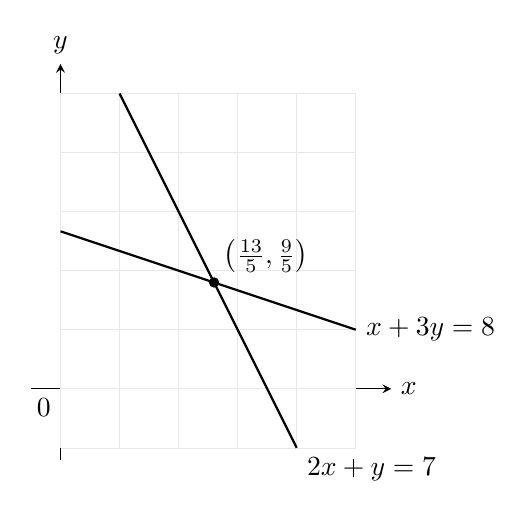
\begin{tikzpicture}[scale=0.75, >=stealth]
    \draw[->] (-0.5,0) -- (5.6,0) node[right] {\(x\)};
    \draw[->] (0,-1.2) -- (0,5.5) node[above] {\(y\)};

    \draw[step=1, gray!18, very thin] (0,-1) grid (5,5);

    \draw[thick] (1,5) -- (4,-1) node[below right] {\(2x+y=7\)};
    \draw[thick] (0,{8/3}) -- (5,1) node[right] {\(x+3y=8\)};

    \fill ({13/5},{9/5}) circle (2.5pt);
    \node[above right] at ({13/5},{9/5}) {\(\left(\frac{13}{5},\frac95\right)\)};

    \node[below left] at (0,0) {\(0\)};
\end{tikzpicture}
\caption{Two independent linear equations in two unknowns meet at one point.}
\end{figure}

We can solve by ordinary elimination.  From
\[
    2x+y=7
\]
we get
\[
    y=7-2x.
\]
Substitute into the second equation:
\[
\begin{aligned}
    x+3(7-2x)&=8,\\
    x+21-6x&=8,\\
    -5x&=-13,
\end{aligned}
\]
so
\[
    x=\frac{13}{5}.
\]
Then
\[
    y=7-2\left(\frac{13}{5}\right)=\frac95.
\]
Thus
\[
\boxed{
    (x,y)=\left(\frac{13}{5},\frac95\right).
}
\]

There is also a column picture.  The two columns
\[
    \mathbf a_1=(2,1),
    \qquad
    \mathbf a_2=(1,3)
\]
span a parallelogram with signed area
\[
    \det
    \begin{pmatrix}
        2&1\\
        1&3
    \end{pmatrix}
    =
    5.
\]
Since this determinant is not zero, the columns are not on one line.  They form a
basis of the plane.  So every output \(\mathbf b\in\mathbb R^2\) has exactly one
description
\[
    \mathbf b=x\mathbf a_1+y\mathbf a_2.
\]

\begin{definition}[Linear system]
A \emph{linear system} is a collection of linear equations in the same unknowns.
For example,
\[
\begin{cases}
2x+y=7,\\
x+3y=8
\end{cases}
\]
is a linear system in the unknowns \(x\) and \(y\).

A \emph{solution} is a choice of the unknowns that satisfies every equation in the
system.
\end{definition}

The matrix
\[
    A=
    \begin{pmatrix}
        2&1\\
        1&3
    \end{pmatrix}
\]
is called the coefficient matrix.  The vector
\[
    \mathbf b=
    \begin{pmatrix}
        7\\8
    \end{pmatrix}
\]
is the right-hand side.

The system is the equation
\[
    A\mathbf x=\mathbf b,
\]
where
\[
    \mathbf x=
    \begin{pmatrix}
        x\\y
    \end{pmatrix}.
\]

\subsection{Three equations and three unknowns}

In three dimensions, each linear equation usually describes a plane.  A solution of
three equations is a point that lies on all three planes.

Consider
\[
\begin{cases}
x+y+z=6,\\
2x-y+z=3,\\
x+2y-z=2.
\end{cases}
\]
We solve by eliminating variables.

Start with the augmented matrix:
\[
\left[
\begin{array}{ccc|c}
1&1&1&6\\
2&-1&1&3\\
1&2&-1&2
\end{array}
\right].
\]
The vertical line separates the coefficient matrix from the right-hand side.

Subtract \(2\) times the first row from the second row:
\[
R_2\leftarrow R_2-2R_1.
\]
Subtract the first row from the third row:
\[
R_3\leftarrow R_3-R_1.
\]
This gives
\[
\left[
\begin{array}{ccc|c}
1&1&1&6\\
0&-3&-1&-9\\
0&1&-2&-4
\end{array}
\right].
\]
Now swap the second and third rows:
\[
\left[
\begin{array}{ccc|c}
1&1&1&6\\
0&1&-2&-4\\
0&-3&-1&-9
\end{array}
\right].
\]
Add \(3\) times the second row to the third:
\[
R_3\leftarrow R_3+3R_2.
\]
Then
\[
\left[
\begin{array}{ccc|c}
1&1&1&6\\
0&1&-2&-4\\
0&0&-7&-21
\end{array}
\right].
\]
The last row says
\[
    -7z=-21,
\]
so
\[
    z=3.
\]
The second row says
\[
    y-2z=-4.
\]
Using \(z=3\),
\[
    y-6=-4,
\]
so
\[
    y=2.
\]
The first row says
\[
    x+y+z=6.
\]
Thus
\[
    x+2+3=6,
\]
so
\[
    x=1.
\]
Therefore
\[
\boxed{
    (x,y,z)=(1,2,3).
}
\]

Geometrically, the three planes meet in one point.

\subsection{Row reduction as organized elimination}

The previous computation used a simple idea: replace the equations by new equations
with the same solutions but fewer variables.

There are three safe moves.

\begin{definition}[Elementary row operations]
The following operations are called \emph{elementary row operations}:

\[
\begin{array}{ll}
1. & \text{Swap two rows.}\\[0.2em]
2. & \text{Multiply a row by a nonzero number.}\\[0.2em]
3. & \text{Add a multiple of one row to another row.}
\end{array}
\]
\end{definition}

These operations do not change the solution set.  They only rewrite the same
information in a more useful form.

\begin{theorem}[Elementary row operations preserve solutions]
If one augmented matrix is obtained from another by elementary row operations, then
the two linear systems have the same solutions.
\end{theorem}

\begin{proof}
Each row is an equation.  Swapping rows only changes the order of the equations.

Multiplying a row by a nonzero number does not change the set of points satisfying
that equation.  For example,
\[
    x+2y=5
\]
and
\[
    3x+6y=15
\]
have the same solutions.

Adding a multiple of one equation to another is reversible.  If we replace
\[
    R_2
\]
by
\[
    R_2+cR_1,
\]
then we can recover the old row by replacing the new row by
\[
    R_2-cR_1.
\]
So no information is lost.
\end{proof}

The word \emph{nonzero} is necessary.  If we multiply an equation by \(0\), we destroy
information.  For example,
\[
    x+y=1
\]
has many solutions, but
\[
    0=0
\]
is satisfied by every point in the plane.  Multiplying by zero has erased the equation.

Row reduction tries to produce a staircase shape.  The first nonzero entry in a row is
called a \emph{pivot}.  Pivots mark variables that are determined by the equations.
Variables without pivots are free to vary.

For the system
\[
\begin{cases}
x+y+z=6,\\
2x-y+z=3,\\
x+2y-z=2,
\end{cases}
\]
the row-reduced form can be pushed all the way to
\[
\left[
\begin{array}{ccc|c}
1&0&0&1\\
0&1&0&2\\
0&0&1&3
\end{array}
\right].
\]
This means
\[
    x=1,\qquad y=2,\qquad z=3.
\]
Every variable has a pivot, so the solution is a single point.

\subsection{Cramer's rule as a geometric formula}

Row reduction is efficient.  But determinants give another formula, one that explains
the geometry.

Return to the two-dimensional system
\[
    x(2,1)+y(1,3)=(7,8).
\]
Let
\[
    \mathbf a_1=(2,1),
    \qquad
    \mathbf a_2=(1,3),
    \qquad
    \mathbf b=(7,8).
\]
The equation is
\[
    x\mathbf a_1+y\mathbf a_2=\mathbf b.
\]

Take the determinant with \(\mathbf a_2\) as the second column:
\[
    \det[\mathbf b\ \mathbf a_2].
\]
Since
\[
    \mathbf b=x\mathbf a_1+y\mathbf a_2,
\]
we get
\[
\begin{aligned}
    \det[\mathbf b\ \mathbf a_2]
    &=
    \det[x\mathbf a_1+y\mathbf a_2\ \ \mathbf a_2]\\
    &=
    x\det[\mathbf a_1\ \mathbf a_2]
    +
    y\det[\mathbf a_2\ \mathbf a_2].
\end{aligned}
\]
But
\[
    \det[\mathbf a_2\ \mathbf a_2]=0
\]
because a parallelogram with two equal sides has zero area.  Therefore
\[
    \det[\mathbf b\ \mathbf a_2]
    =
    x\det[\mathbf a_1\ \mathbf a_2].
\]
So
\[
\boxed{
    x=
    \frac{\det[\mathbf b\ \mathbf a_2]}
         {\det[\mathbf a_1\ \mathbf a_2]}.
}
\]

Similarly,
\[
\boxed{
    y=
    \frac{\det[\mathbf a_1\ \mathbf b]}
         {\det[\mathbf a_1\ \mathbf a_2]}.
}
\]

In our example,
\[
    \det[\mathbf a_1\ \mathbf a_2]
    =
    \det
    \begin{pmatrix}
        2&1\\
        1&3
    \end{pmatrix}
    =
    5.
\]
Then
\[
    x
    =
    \frac{
    \det
    \begin{pmatrix}
        7&1\\
        8&3
    \end{pmatrix}}
    {5}
    =
    \frac{21-8}{5}
    =
    \frac{13}{5},
\]
and
\[
    y
    =
    \frac{
    \det
    \begin{pmatrix}
        2&7\\
        1&8
    \end{pmatrix}}
    {5}
    =
    \frac{16-7}{5}
    =
    \frac95.
\]

\begin{theorem}[Cramer's rule in the plane]
Let
\[
    A=
    \begin{pmatrix}
        a&b\\
        c&d
    \end{pmatrix},
    \qquad
    \mathbf b=
    \begin{pmatrix}
        r\\s
    \end{pmatrix}.
\]
If
\[
    \det A\neq0,
\]
then the system
\[
    A
    \begin{pmatrix}
        x\\y
    \end{pmatrix}
    =
    \mathbf b
\]
has the unique solution
\[
\boxed{
    x=
    \frac{
    \det
    \begin{pmatrix}
        r&b\\
        s&d
    \end{pmatrix}}
    {\det A},
    \qquad
    y=
    \frac{
    \det
    \begin{pmatrix}
        a&r\\
        c&s
    \end{pmatrix}}
    {\det A}.
}
\]
\end{theorem}

Cramer's rule also works in space.  If
\[
    \mathbf b=x\mathbf a_1+y\mathbf a_2+z\mathbf a_3,
\]
then
\[
\boxed{
    x=
    \frac{\det[\mathbf b\ \mathbf a_2\ \mathbf a_3]}
         {\det[\mathbf a_1\ \mathbf a_2\ \mathbf a_3]},
}
\]
\[
\boxed{
    y=
    \frac{\det[\mathbf a_1\ \mathbf b\ \mathbf a_3]}
         {\det[\mathbf a_1\ \mathbf a_2\ \mathbf a_3]},
}
\]
and
\[
\boxed{
    z=
    \frac{\det[\mathbf a_1\ \mathbf a_2\ \mathbf b]}
         {\det[\mathbf a_1\ \mathbf a_2\ \mathbf a_3]}.
}
\]
The proof is the same, with signed volume replacing signed area.

Cramer's rule is not usually the fastest way to solve a large system.  Row reduction is
better for computation.  But Cramer's rule reveals the geometry: the coefficient of a
column is found by comparing signed areas or signed volumes.

\subsection{When there is no solution, one solution, or many solutions}

A linear system has only three possible behaviors:
\[
    \text{no solution},\qquad
    \text{one solution},\qquad
    \text{many solutions}.
\]
There is no fourth option.

Two lines in the plane show all three possibilities.

\begin{example}[One solution]
The system
\[
\begin{cases}
2x+y=7,\\
x+3y=8
\end{cases}
\]
has one solution:
\[
    (x,y)=\left(\frac{13}{5},\frac95\right).
\]
The two lines cross in one point.  The coefficient determinant is nonzero:
\[
    \det
    \begin{pmatrix}
        2&1\\
        1&3
    \end{pmatrix}
    =
    5.
\]
\end{example}

\begin{example}[No solution]
The system
\[
\begin{cases}
x+y=1,\\
2x+2y=5
\end{cases}
\]
has no solution.

The second left-hand side is twice the first:
\[
    2x+2y=2(x+y).
\]
If \(x+y=1\), then \(2x+2y=2\), not \(5\).  Row reduction shows the contradiction:
\[
\left[
\begin{array}{cc|c}
1&1&1\\
2&2&5
\end{array}
\right]
\longrightarrow
\left[
\begin{array}{cc|c}
1&1&1\\
0&0&3
\end{array}
\right].
\]
The last row says
\[
    0=3,
\]
which is impossible.

Geometrically, the two lines are parallel and distinct.
\end{example}

\begin{example}[Many solutions]
The system
\[
\begin{cases}
x+y=1,\\
2x+2y=2
\end{cases}
\]
has many solutions.

The second equation is just twice the first.  Row reduction gives
\[
\left[
\begin{array}{cc|c}
1&1&1\\
2&2&2
\end{array}
\right]
\longrightarrow
\left[
\begin{array}{cc|c}
1&1&1\\
0&0&0
\end{array}
\right].
\]
Only one real equation remains:
\[
    x+y=1.
\]
Let
\[
    y=t.
\]
Then
\[
    x=1-t.
\]
So all solutions are
\[
\boxed{
    (x,y)=(1-t,t),\qquad t\in\mathbb R.
}
\]
Geometrically, the two equations describe the same line.
\end{example}

The same pattern appears in space.  Three planes can meet in a point, miss each other,
or share a line or plane.

\begin{example}[A line of solutions in space]
Consider
\[
\begin{cases}
x+y+z=4,\\
x-y+z=2.
\end{cases}
\]
Subtract the second equation from the first:
\[
    2y=2,
\]
so
\[
    y=1.
\]
Then
\[
    x+z=3.
\]
Let
\[
    z=t.
\]
Then
\[
    x=3-t.
\]
The solutions are
\[
\boxed{
    (x,y,z)=(3-t,1,t),\qquad t\in\mathbb R.
}
\]
This is a line.  Geometrically, two nonparallel planes in space usually intersect in a
line.
\end{example}

The determinant gives the cleanest test for square systems.

\begin{theorem}[Nonzero determinant gives one solution]
Let \(A\) be an \(n\times n\) matrix, with \(n=2\) or \(n=3\).  If
\[
    \det A\neq0,
\]
then for every right-hand side \(\mathbf b\), the system
\[
    A\mathbf x=\mathbf b
\]
has exactly one solution.
\end{theorem}

\begin{proof}
When \(\det A\neq0\), the linear transformation
\[
    \mathbf x\longmapsto A\mathbf x
\]
does not collapse area in the plane or volume in space.  Its columns form a basis of
the output space.  Therefore every output \(\mathbf b\) has a unique coordinate
description in those columns:
\[
    \mathbf b=x_1\mathbf a_1+\cdots+x_n\mathbf a_n.
\]
Those coordinates are the unique solution of
\[
    A\mathbf x=\mathbf b.
\]
\end{proof}

The hypothesis
\[
    \det A\neq0
\]
is essential.

For example, let
\[
    A=
    \begin{pmatrix}
        1&1\\
        2&2
    \end{pmatrix}.
\]
Then
\[
    \det A=0.
\]
The system
\[
    A
    \begin{pmatrix}
        x\\y
    \end{pmatrix}
    =
    \begin{pmatrix}
        1\\2
    \end{pmatrix}
\]
has many solutions, because it is just
\[
    x+y=1.
\]
But the system
\[
    A
    \begin{pmatrix}
        x\\y
    \end{pmatrix}
    =
    \begin{pmatrix}
        1\\5
    \end{pmatrix}
\]
has no solution, because it says
\[
    x+y=1
\]
and
\[
    2x+2y=5
\]
at the same time.

So determinant zero does not mean one specific failure.  It means collapse.  Once a
machine collapses the plane or space, some outputs are unreachable and some reachable
outputs come from many inputs.

Linear systems are about flat objects: lines, planes, and hyperplanes.  But calculus will
soon ask about curved objects.  Near a point, a curved surface first looks like a plane;
that is the linear part.  When the plane becomes horizontal and the first-order change
vanishes, the next visible shape is quadratic.  A bowl, a dome, and a saddle all begin
with expressions like
\[
    ax^2+bxy+cy^2.
\]
To read those shapes, we need one more matrix idea.

\section{Quadratic forms and symmetric matrices}
\label{sec:3.6}

Linear equations gave us flat geometry.  A line, a plane, and a hyperplane all come from
first powers of the variables.  The next layer of geometry comes from second powers:
\[
    x^2,\qquad xy,\qquad y^2.
\]
This is where bowls, domes, ellipses, hyperbolas, and saddle points first appear.

\subsection{From \(ax^2+bxy+cy^2\) to matrices}

Picture a shallow metal dish whose height above a flat table is
\[
    q(x,y)=5x^2+4xy+2y^2.
\]
The cross term
\[
    4xy
\]
means the dish is not aligned with the \(x\)- and \(y\)-axes.  It is tilted relative to
the coordinate grid.

The expression can be written with a matrix:
\[
\begin{aligned}
    q(x,y)
    &=
    \begin{pmatrix}x&y\end{pmatrix}
    \begin{pmatrix}
        5&2\\
        2&2
    \end{pmatrix}
    \begin{pmatrix}
        x\\y
    \end{pmatrix}.
\end{aligned}
\]
Check the multiplication:
\[
    \begin{pmatrix}
        5&2\\
        2&2
    \end{pmatrix}
    \begin{pmatrix}
        x\\y
    \end{pmatrix}
    =
    \begin{pmatrix}
        5x+2y\\
        2x+2y
    \end{pmatrix}.
\]
Then
\[
\begin{aligned}
    \begin{pmatrix}x&y\end{pmatrix}
    \begin{pmatrix}
        5x+2y\\
        2x+2y
    \end{pmatrix}
    &=
    x(5x+2y)+y(2x+2y)\\
    &=
    5x^2+4xy+2y^2.
\end{aligned}
\]
The off-diagonal entries both contribute to the \(xy\)-term:
\[
    2xy+2xy=4xy.
\]

\begin{definition}[Quadratic form in two variables]
A \emph{quadratic form} in two variables is a function
\[
    q:\mathbb R^2\to\mathbb R
\]
of the form
\[
    q(x,y)=ax^2+bxy+cy^2.
\]
It can be written as
\[
\boxed{
    q(x,y)
    =
    \begin{pmatrix}x&y\end{pmatrix}
    \begin{pmatrix}
        a&b/2\\
        b/2&c
    \end{pmatrix}
    \begin{pmatrix}
        x\\y
    \end{pmatrix}.
}
\]
\end{definition}

The matrix
\[
    \begin{pmatrix}
        a&b/2\\
        b/2&c
    \end{pmatrix}
\]
is symmetric: its entries mirror across the diagonal.

\begin{definition}[Symmetric matrix]
A square matrix \(A\) is \emph{symmetric} if
\[
    A^T=A.
\]
For a \(2\times2\) matrix, this means
\[
    A=
    \begin{pmatrix}
        a&b\\
        b&c
    \end{pmatrix}.
\]
\end{definition}

Symmetric matrices are the natural matrices for quadratic forms.  To see why, try a
matrix that is not symmetric:
\[
    M=
    \begin{pmatrix}
        5&4\\
        0&2
    \end{pmatrix}.
\]
Then
\[
\begin{aligned}
    \begin{pmatrix}x&y\end{pmatrix}
    M
    \begin{pmatrix}
        x\\y
    \end{pmatrix}
    &=
    \begin{pmatrix}x&y\end{pmatrix}
    \begin{pmatrix}
        5x+4y\\
        2y
    \end{pmatrix}\\
    &=
    5x^2+4xy+2y^2.
\end{aligned}
\]
This is the same quadratic form as before.  The nonsymmetric matrix \(M\) did not add
a new quadratic form.

Its symmetric part is
\[
    \frac12(M+M^T)
    =
    \frac12
    \left(
    \begin{pmatrix}
        5&4\\
        0&2
    \end{pmatrix}
    +
    \begin{pmatrix}
        5&0\\
        4&2
    \end{pmatrix}
    \right)
    =
    \begin{pmatrix}
        5&2\\
        2&2
    \end{pmatrix}.
\]

\begin{theorem}[Only the symmetric part matters]
For any square matrix \(M\) and any vector \(\mathbf x\),
\[
\boxed{
    \mathbf x^T M\mathbf x
    =
    \mathbf x^T\left(\frac{M+M^T}{2}\right)\mathbf x.
}
\]
\end{theorem}

\begin{proof}
Split \(M\) into two pieces:
\[
    M=
    \frac{M+M^T}{2}
    +
    \frac{M-M^T}{2}.
\]
The first piece is symmetric.  The second piece is skew-symmetric, meaning its
transpose is its negative.

Let
\[
    K=\frac{M-M^T}{2}.
\]
Then
\[
    K^T=-K.
\]
The number
\[
    \mathbf x^TK\mathbf x
\]
is a \(1\times1\) matrix, so it equals its own transpose:
\[
    \mathbf x^TK\mathbf x
    =
    (\mathbf x^TK\mathbf x)^T
    =
    \mathbf x^TK^T\mathbf x
    =
    -\mathbf x^TK\mathbf x.
\]
Therefore
\[
    \mathbf x^TK\mathbf x=0.
\]
So only the symmetric part contributes.
\end{proof}

The hypothesis that we use the symmetric part is not cosmetic.  For example,
\[
    K=
    \begin{pmatrix}
        0&10\\
        -10&0
    \end{pmatrix}
\]
has determinant \(100\), but
\[
    \begin{pmatrix}x&y\end{pmatrix}
    K
    \begin{pmatrix}
        x\\y
    \end{pmatrix}
    =
    \begin{pmatrix}x&y\end{pmatrix}
    \begin{pmatrix}
        10y\\
        -10x
    \end{pmatrix}
    =
    10xy-10xy
    =
    0
\]
for every \((x,y)\).  As a linear transformation, \(K\) rotates and scales.  As a
quadratic form, it contributes nothing.  That is why quadratic forms belong to
symmetric matrices.

Despite the name, a quadratic form is not the same thing as a differential form.  A
quadratic form takes one vector and returns a number that scales like the square of the
input:
\[
    q(c\mathbf v)=c^2q(\mathbf v).
\]
Differential forms later will be linear, alternating measuring rules used as integrands.
The shared word \emph{form} means ``a rule with algebraic structure,'' but the structures
are different.

\subsection{Ellipses, hyperbolas, and rotated axes}

The quadratic form
\[
    q(x,y)=5x^2+4xy+2y^2
\]
is always positive except at the origin.  One way to see this is to complete the square:
\[
\begin{aligned}
    q(x,y)
    &=
    5x^2+4xy+2y^2\\
    &=
    5\left(x+\frac25y\right)^2+\frac65y^2.
\end{aligned}
\]
Both terms are nonnegative, and both are zero only when
\[
    x=0,\qquad y=0.
\]
So the graph
\[
    z=q(x,y)
\]
is a bowl.

The level curves
\[
    q(x,y)=c
\]
for \(c>0\) are ellipses.  But they are rotated ellipses, because of the cross term
\(4xy\).

A better coordinate system reveals the shape.  Let
\[
    \mathbf p=\frac1{\sqrt5}(2,1),
    \qquad
    \mathbf r=\frac1{\sqrt5}(1,-2).
\]
These are perpendicular unit vectors.  Use them as new axes:
\[
    (x,y)=u\mathbf p+v\mathbf r.
\]
That means
\[
    x=\frac{2u+v}{\sqrt5},
    \qquad
    y=\frac{u-2v}{\sqrt5}.
\]
Substituting into \(q\) gives
\[
\boxed{
    q(x,y)=6u^2+v^2.
}
\]
In the rotated coordinates, the cross term disappears.  The level curve
\[
    q(x,y)=1
\]
becomes
\[
    6u^2+v^2=1,
\]
which is an ellipse aligned with the \(u\)- and \(v\)-axes.

\begin{figure}[h]
\centering
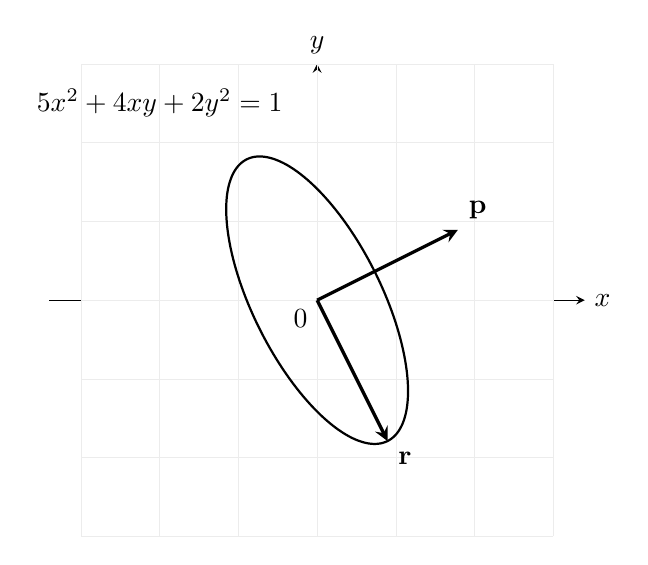
\begin{tikzpicture}[scale=2.0, >=stealth]
    \draw[->] (-1.7,0) -- (1.7,0) node[right] {\(x\)};
    \draw[->] (0,-1.5) -- (0,1.5) node[above] {\(y\)};

    \draw[step=0.5, gray!15, very thin] (-1.5,-1.5) grid (1.5,1.5);

    \draw[thick, domain=0:360, samples=160, variable=\t]
        plot ({(2*(cos(\t)/sqrt(6))+sin(\t))/sqrt(5)},
              {((cos(\t)/sqrt(6))-2*sin(\t))/sqrt(5)});

    \draw[->, very thick] (0,0) -- ({2/sqrt(5)},{1/sqrt(5)}) node[above right] {\(\mathbf p\)};
    \draw[->, very thick] (0,0) -- ({1/sqrt(5)},{-2/sqrt(5)}) node[below right] {\(\mathbf r\)};

    \node at (-1.0,1.25) {\(5x^2+4xy+2y^2=1\)};
    \node[below left] at (0,0) {\(0\)};
\end{tikzpicture}
\caption{The cross term \(4xy\) rotates the ellipse.  In the right axes, it becomes
\(6u^2+v^2=1\).}
\end{figure}

The same idea explains hyperbolas.  Consider
\[
    q(x,y)=2xy.
\]
This has only a cross term.  Use the rotated coordinates
\[
    u=\frac{x+y}{\sqrt2},
    \qquad
    v=\frac{x-y}{\sqrt2}.
\]
Solving for \(x\) and \(y\),
\[
    x=\frac{u+v}{\sqrt2},
    \qquad
    y=\frac{u-v}{\sqrt2}.
\]
Then
\[
\begin{aligned}
    2xy
    &=
    2\left(\frac{u+v}{\sqrt2}\right)
      \left(\frac{u-v}{\sqrt2}\right)\\
    &=
    u^2-v^2.
\end{aligned}
\]
So
\[
    2xy=1
\]
is the rotated version of
\[
    u^2-v^2=1,
\]
a hyperbola.

The graph
\[
    z=2xy
\]
is a saddle.  Along the line \(y=x\),
\[
    z=2x^2,
\]
so the surface curves upward.  Along the line \(y=-x\),
\[
    z=-2x^2,
\]
so the surface curves downward.

The same point is both valley-like and ridge-like, depending on the direction.

\subsection{Positive definite, negative definite, and indefinite forms}

A quadratic form can have different sign patterns.

\begin{definition}[Definite and indefinite quadratic forms]
Let
\[
    q(\mathbf x)=\mathbf x^TA\mathbf x
\]
be a quadratic form.

\[
\begin{array}{ll}
q \text{ is positive definite} &
\text{if } q(\mathbf x)>0 \text{ for every } \mathbf x\neq\mathbf 0.\\[0.4em]
q \text{ is negative definite} &
\text{if } q(\mathbf x)<0 \text{ for every } \mathbf x\neq\mathbf 0.\\[0.4em]
q \text{ is indefinite} &
\text{if } q \text{ takes both positive and negative values.}
\end{array}
\]
\end{definition}

The pictures are memorable:

\[
\begin{array}{c|c|c}
\text{Type} & \text{Example} & \text{Shape of }z=q(x,y)\\ \hline
\text{positive definite} & x^2+y^2 & \text{bowl}\\
\text{negative definite} & -x^2-y^2 & \text{dome}\\
\text{indefinite} & x^2-y^2 & \text{saddle}
\end{array}
\]

There is also a borderline case.  The form
\[
    q(x,y)=(2x+y)^2
\]
is never negative, but it is zero along the whole line
\[
    2x+y=0.
\]
So it is not positive definite.  It has a flat direction.

For \(2\times2\) symmetric matrices, there is a simple determinant test.

\begin{theorem}[The \(2\times2\) quadratic-form test]
Let
\[
    A=
    \begin{pmatrix}
        a&b\\
        b&c
    \end{pmatrix}
\]
be symmetric, and let
\[
    q(x,y)=
    \begin{pmatrix}x&y\end{pmatrix}
    A
    \begin{pmatrix}
        x\\y
    \end{pmatrix}
    =
    ax^2+2bxy+cy^2.
\]
Let
\[
    \Delta=\det A=ac-b^2.
\]
Then:

\[
\begin{array}{ll}
1. & q \text{ is positive definite if and only if } a>0 \text{ and } \Delta>0.\\[0.3em]
2. & q \text{ is negative definite if and only if } a<0 \text{ and } \Delta>0.\\[0.3em]
3. & q \text{ is indefinite if } \Delta<0.
\end{array}
\]
\end{theorem}

\begin{proof}
Assume first that \(a\neq0\).  Complete the square:
\[
\begin{aligned}
    q(x,y)
    &=
    ax^2+2bxy+cy^2\\
    &=
    a\left(x+\frac ba y\right)^2
    +
    \left(c-\frac{b^2}{a}\right)y^2\\
    &=
    a\left(x+\frac ba y\right)^2
    +
    \frac{ac-b^2}{a}y^2\\
    &=
    a\left(x+\frac ba y\right)^2
    +
    \frac{\Delta}{a}y^2.
\end{aligned}
\]

If \(a>0\) and \(\Delta>0\), then both coefficients are positive.  The form is positive
except at the origin.

If \(a<0\) and \(\Delta>0\), then both coefficients are negative.  The form is negative
except at the origin.

If \(\Delta<0\) and \(a\neq0\), then the two square terms have opposite signs.  The
form takes both positive and negative values, so it is indefinite.

If \(a=0\) and \(\Delta<0\), then
\[
    \Delta=-b^2<0,
\]
so \(b\neq0\).  In that case
\[
    q(x,y)=2bxy+cy^2.
\]
Taking \(y=1\), the expression
\[
    q(x,1)=2bx+c
\]
takes both positive and negative values as \(x\) varies.  So \(q\) is indefinite.
\end{proof}

Each condition matters.

First, \(\Delta>0\) alone does not mean positive definite.  The matrix
\[
    A=
    \begin{pmatrix}
        -1&0\\
        0&-1
    \end{pmatrix}
\]
has
\[
    \det A=1>0,
\]
but
\[
    q(x,y)=-x^2-y^2
\]
is negative definite, not positive definite.  We also need the sign of \(a\).

Second, \(a>0\) alone does not mean positive definite.  The matrix
\[
    A=
    \begin{pmatrix}
        1&0\\
        0&-1
    \end{pmatrix}
\]
has
\[
    a=1>0,
\]
but
\[
    q(x,y)=x^2-y^2
\]
takes both signs.  The determinant is
\[
    \det A=-1<0,
\]
and the form is indefinite.

Third, when
\[
    \Delta=0,
\]
there is a flat direction.  For example,
\[
    q(x,y)=(2x+y)^2
\]
has matrix
\[
    A=
    \begin{pmatrix}
        4&2\\
        2&1
    \end{pmatrix},
\]
and
\[
    \det A=4\cdot1-2\cdot2=0.
\]
The form is not positive definite because
\[
    q(1,-2)=0
\]
even though
\[
    (1,-2)\neq(0,0).
\]

The determinant has returned as a collapse detector.  For a linear transformation,
\(\det A=0\) meant area was collapsed.  For a quadratic form, \(\det A=0\) means one
curvature direction has flattened.

\subsection{Preview: the Hessian matrix will classify critical points}

Quadratic forms matter in calculus because a curved function often looks quadratic
after its linear part disappears.

Suppose a hiker stands at a point on a hill where the tangent plane is horizontal.
There is no first-order uphill direction at that exact point.  The next question is not
``Which way is the slope?''  The slope starts at zero.  The next question is:

\[
    \text{Does the surface bend up, bend down, or bend both ways?}
\]

That bending is measured by a quadratic form.

Later, near a point \((a,b)\), a function \(f(x,y)\) will have an approximation of the
form
\[
    f(a+h,b+k)
    \approx
    f(a,b)
    +
    \text{linear part}
    +
    \frac12
    \begin{pmatrix}h&k\end{pmatrix}
    H
    \begin{pmatrix}
        h\\k
    \end{pmatrix}.
\]
The matrix
\[
    H=
    \begin{pmatrix}
        f_{xx}&f_{xy}\\
        f_{yx}&f_{yy}
    \end{pmatrix}
\]
is called the Hessian matrix.

At a critical point, the linear part is zero.  Then the Hessian's quadratic form becomes
the first visible shape:

\[
\begin{array}{c|c}
\text{Hessian type} & \text{Local shape} \\ \hline
\text{positive definite} & \text{local minimum, like a bowl}\\
\text{negative definite} & \text{local maximum, like a dome}\\
\text{indefinite} & \text{saddle point}\\
\text{degenerate} & \text{the quadratic part is not enough}
\end{array}
\]

This is only a preview.  We do not yet have the derivative of a multivariable function.
But the pattern is now visible: matrices describe the best linear part, and symmetric
matrices describe the first curved part.  The next step is to make the phrase
``best linear part'' precise.  That phrase will become the multivariable derivative.
\section{Linear approximation as a preview of the derivative}
\label{sec:3.7}

Section 3.6 ended with the phrase \emph{best linear part}.  That phrase is the reason
Chapter 3 belongs in a calculus book.  Matrices are not only a way to solve systems.
They are the language of what a curved function looks like when we zoom in close
enough.

A curve may bend.  A surface may bend in many directions.  But at a small enough
scale, the first visible piece is often linear.

\subsection{A curved function looks linear when viewed very close}

Suppose a cyclist rides along a mountain road.  Let \(t\) be distance along the road,
measured in kilometers from a marker, and let
\[
    H(t)=20+6t-\frac12 t^2
\]
be the altitude in meters above some reference level.

At \(t=4\),
\[
    H(4)=20+24-8=36.
\]
Now move a small amount \(h\) farther along the road.  The new altitude is
\[
\begin{aligned}
H(4+h)
&=
20+6(4+h)-\frac12(4+h)^2\\
&=
20+24+6h-\frac12(16+8h+h^2)\\
&=
36+2h-\frac12h^2.
\end{aligned}
\]
So the change in altitude is
\[
    H(4+h)-H(4)=2h-\frac12h^2.
\]

The term
\[
    2h
\]
is linear in the displacement \(h\).  The term
\[
    -\frac12h^2
\]
is quadratic.  If \(h\) is small, the quadratic term is much smaller than the linear
term.

For example:
\[
\begin{array}{c|c|c}
h & 2h & -\frac12h^2 \\ \hline
0.1 & 0.2 & -0.005\\
0.01 & 0.02 & -0.00005\\
0.001 & 0.002 & -0.0000005
\end{array}
\]
The closer we zoom to \(t=4\), the more the change looks like
\[
    H(4+h)-H(4)\approx 2h.
\]
Equivalently,
\[
    H(4+h)\approx 36+2h.
\]

\begin{figure}[h]
\centering
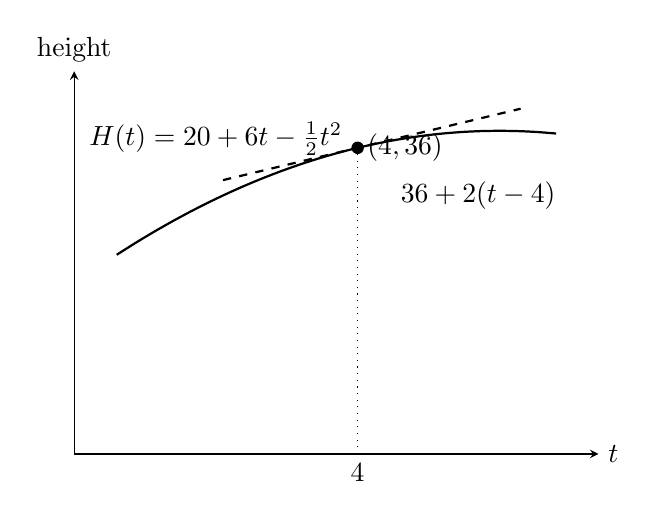
\begin{tikzpicture}[scale=0.9, >=stealth]
    \draw[->] (0,0) -- (7.4,0) node[right] {\(t\)};
    \draw[->] (0,0) -- (0,5.4) node[above] {height};

    \draw[domain=0.6:6.8, smooth, variable=\t, thick]
        plot ({\t},{0.12*(20+6*\t-0.5*\t*\t)});

    \draw[domain=2.1:6.3, smooth, variable=\t, thick, dashed]
        plot ({\t},{0.12*(28+2*\t)});

    \fill (4,{0.12*36}) circle (2.5pt);
    \draw[dotted] (4,0) -- (4,{0.12*36});
    \node[below] at (4,0) {\(4\)};
    \node[right] at (4,{0.12*36}) {\((4,36)\)};

    \node at (2.0,4.45) {\(H(t)=20+6t-\frac12t^2\)};
    \node at (5.7,3.65) {\(36+2(t-4)\)};
\end{tikzpicture}
\caption{Near \(t=4\), the curved altitude graph is well approximated by a line.}
\end{figure}

The line
\[
    36+2h
\]
has two parts:
\[
    \underbrace{36}_{\text{starting value}}
    +
    \underbrace{2h}_{\text{linear change}}.
\]
The derivative is the linear-change part:
\[
    h\longmapsto 2h.
\]
In single-variable calculus, we often store this information as the number
\[
    H'(4)=2.
\]
But for the multivariable story, it is better to think of the derivative as the linear
function
\[
    L(h)=2h.
\]

This small shift in viewpoint is important.  In one variable, a linear function is just
multiplication by a number.  In several variables, a linear function or linear
transformation may need a whole matrix.

\subsection{The derivative as the best linear map}

Now imagine a gently curved roof.  Near one support beam, choose coordinates so that
the beam is at the origin.  Suppose the height of the roof is
\[
    f(x,y)=12+3x-2y+\frac14x^2-\frac12xy+\frac18y^2.
\]
At the origin,
\[
    f(0,0)=12.
\]
For a small displacement
\[
    (h,k),
\]
we have
\[
\begin{aligned}
f(h,k)
&=
12+3h-2k+\frac14h^2-\frac12hk+\frac18k^2\\
&=
12+\underbrace{(3h-2k)}_{\text{linear part}}
+
\underbrace{\left(\frac14h^2-\frac12hk+\frac18k^2\right)}_{\text{quadratic error}}.
\end{aligned}
\]
So near the origin,
\[
    f(h,k)\approx 12+3h-2k.
\]
The tangent plane preview is
\[
    z=12+3x-2y.
\]

But the derivative is not the whole affine expression
\[
    12+3h-2k.
\]
The derivative is only the linear change:
\[
    L(h,k)=3h-2k.
\]
In the language of Chapter 3,
\[
    L:\mathbb R^2\to\mathbb R
\]
is a linear function.  By Section 3.1, it is a dot product:
\[
    L(h,k)=(3,-2)\cdot(h,k).
\]

Using the component-reading forms from Chapter 2, we can also write the same linear
function as
\[
    L=3\,dx-2\,dy.
\]
This means
\[
    L(h,k)=3\,dx(h,k)-2\,dy(h,k)=3h-2k.
\]
Later, this linear function will be called the \emph{differential} of \(f\) at the origin,
and we will write
\[
    df=3\,dx-2\,dy
\]
at that point.

For now, the main idea is this:

\[
\boxed{
\text{A derivative is the best linear rule for predicting small changes.}
}
\]

\begin{definition}[Best linear approximation, preview]
Let
\[
    F:\mathbb R^n\to\mathbb R^m
\]
be a function, and let \(\mathbf a\in\mathbb R^n\).  A linear map
\[
    L:\mathbb R^n\to\mathbb R^m
\]
is the \emph{best linear approximation} to \(F\) at \(\mathbf a\) if
\[
    F(\mathbf a+\mathbf h)
    =
    F(\mathbf a)+L(\mathbf h)+\text{error}
\]
and the error becomes small compared with \(\|\mathbf h\|\) as
\[
    \mathbf h\to\mathbf 0.
\]
In symbols,
\[
    \frac{\|\text{error}\|}{\|\mathbf h\|}\to0.
\]

When such an \(L\) exists, it is called the \emph{derivative} of \(F\) at \(\mathbf a\),
and is written
\[
    DF(\mathbf a).
\]
\end{definition}

The phrase ``small compared with \(\|\mathbf h\|\)'' is the important part.  It says the
error is not merely small.  It is smaller than first-order size.

\begin{theorem}[The best linear part is unique]
If a function
\[
    F:\mathbb R^n\to\mathbb R^m
\]
has a best linear approximation at \(\mathbf a\), then that linear approximation is
unique.
\end{theorem}

\begin{proof}
Suppose two linear maps \(L\) and \(M\) both work.  Then
\[
    F(\mathbf a+\mathbf h)
    =
    F(\mathbf a)+L(\mathbf h)+\mathbf r_L(\mathbf h)
\]
and
\[
    F(\mathbf a+\mathbf h)
    =
    F(\mathbf a)+M(\mathbf h)+\mathbf r_M(\mathbf h),
\]
where both errors are small compared with \(\|\mathbf h\|\).

Subtract the two equations:
\[
    (L-M)(\mathbf h)=\mathbf r_M(\mathbf h)-\mathbf r_L(\mathbf h).
\]
Now choose any unit vector \(\mathbf u\), and set
\[
    \mathbf h=t\mathbf u.
\]
Because \(L-M\) is linear,
\[
    (L-M)(t\mathbf u)=t(L-M)(\mathbf u).
\]
Dividing by \(|t|\), the left side has size
\[
    \|(L-M)(\mathbf u)\|.
\]
The right side tends to \(0\), because both errors are small compared with
\(\|\mathbf h\|=|t|\).  Therefore
\[
    (L-M)(\mathbf u)=\mathbf 0.
\]
This holds for every unit vector \(\mathbf u\), so
\[
    L=M.
\]
\end{proof}

The condition on the error is necessary.  If we only required the error to go to zero,
the zero function
\[
    F(h)=0
\]
would have many ``linear approximations'' at the origin.  For example,
\[
    L(h)=0
\]
and
\[
    M(h)=7h
\]
would both give errors that go to zero as \(h\to0\).  But \(M\) is not a first-order
approximation to the zero function, because its error
\[
    -7h
\]
is the same size as \(h\), not smaller.

So the derivative is not just a nearby linear rule.  It is the linear rule that captures all
first-order change.

\begin{example}[A cone has no best linear part at its tip]
Consider
\[
    c(x,y)=\sqrt{x^2+y^2}.
\]
This is the height of a cone whose tip is at the origin.

The function is continuous at the origin:
\[
    c(x,y)\to0
    \qquad\text{as}\qquad
    (x,y)\to(0,0).
\]
But it has no best linear approximation there.

To see why, restrict to the \(x\)-axis.  Along points \((h,0)\),
\[
    c(h,0)=|h|.
\]
If \(c\) had a linear approximation \(L\) at the origin, then along the \(x\)-axis it would
look like
\[
    L(h,0)=ah
\]
for some number \(a\).

For \(h>0\), the approximation to \(|h|\) would force
\[
    a=1.
\]
For \(h<0\), it would force
\[
    a=-1.
\]
No single number \(a\) can do both.

The cone is not failing because it is discontinuous.  It is failing because the tip has a
corner.  When we zoom in, the corner remains a corner; it never becomes a plane.
\end{example}

This is the first warning for multivariable derivatives.  A function can be continuous
and still fail to have a linear part.

\subsection{Why matrices appear in multivariable differentiation}

Scalar-valued functions produce one linear function as their derivative.  Vector-valued
functions produce a linear transformation, and therefore a matrix.

Consider the nonlinear transformation
\[
    F:\mathbb R^2\to\mathbb R^2
\]
given by
\[
    F(s,t)=
    \bigl(2s+t+s^2,\;s-3t+st\bigr).
\]
We study it near the point
\[
    (1,2).
\]
Write a nearby input as
\[
    (s,t)=(1+h,2+k).
\]
Then
\[
\begin{aligned}
F(1+h,2+k)
&=
\bigl(2(1+h)+(2+k)+(1+h)^2,\;
(1+h)-3(2+k)+(1+h)(2+k)\bigr)\\
&=
\bigl(5+4h+k+h^2,\;-3+3h-2k+hk\bigr).
\end{aligned}
\]
So
\[
    F(1+h,2+k)
    =
    (5,-3)
    +
    (4h+k,\;3h-2k)
    +
    (h^2,hk).
\]
The first term is the starting output:
\[
    F(1,2)=(5,-3).
\]
The second term is linear in \((h,k)\):
\[
    (h,k)\longmapsto (4h+k,\;3h-2k).
\]
The last term is quadratic error:
\[
    (h^2,hk).
\]

The derivative is therefore the linear transformation
\[
    DF(1,2)(h,k)=(4h+k,\;3h-2k).
\]
Its matrix is
\[
\boxed{
    DF(1,2)=
    \begin{pmatrix}
        4&1\\
        3&-2
    \end{pmatrix}.
}
\]

This matrix has the same two readings as every matrix from Section 3.2.

The rows are the linear functions that give the output coordinates:
\[
    4h+k,
    \qquad
    3h-2k.
\]
The columns are the images of the basic small input directions:
\[
    \begin{pmatrix}4\\3\end{pmatrix},
    \qquad
    \begin{pmatrix}1\\-2\end{pmatrix}.
\]

So a tiny square in the input plane, placed near \((1,2)\), is sent approximately to the
parallelogram spanned by these two columns.

\begin{figure}[h]
\centering
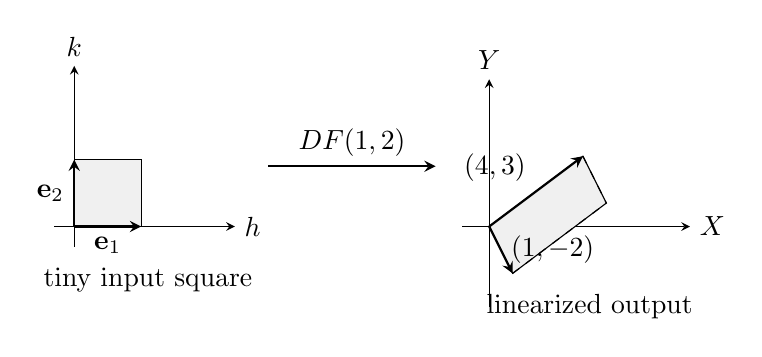
\begin{tikzpicture}[scale=0.85, >=stealth]
    \begin{scope}
        \draw[->] (-0.3,0) -- (2.4,0) node[right] {\(h\)};
        \draw[->] (0,-0.3) -- (0,2.4) node[above] {\(k\)};
        \draw[fill=gray!12] (0,0) -- (1,0) -- (1,1) -- (0,1) -- cycle;
        \draw[->, thick] (0,0) -- (1,0) node[midway, below] {\(\mathbf e_1\)};
        \draw[->, thick] (0,0) -- (0,1) node[midway, left] {\(\mathbf e_2\)};
        \node at (1.1,-0.8) {tiny input square};
    \end{scope}

    \begin{scope}[shift={(6.2,0)}]
        \draw[->] (-0.4,0) -- (3.0,0) node[right] {\(X\)};
        \draw[->] (0,-1.2) -- (0,2.2) node[above] {\(Y\)};

        \coordinate (O) at (0,0);
        \coordinate (U) at (1.4,1.05);
        \coordinate (V) at (0.35,-0.7);
        \coordinate (UV) at (1.75,0.35);

        \draw[fill=gray!12] (O) -- (U) -- (UV) -- (V) -- cycle;
        \draw[->, thick] (O) -- (U) node[midway, above left] {\((4,3)\)};
        \draw[->, thick] (O) -- (V) node[midway, right] {\((1,-2)\)};
        \draw[dashed] (U) -- (UV);
        \draw[dashed] (V) -- (UV);
        \node at (1.5,-1.2) {linearized output};
    \end{scope}

    \draw[->, thick] (2.9,0.9) -- (5.4,0.9) node[midway, above] {\(DF(1,2)\)};
\end{tikzpicture}
\caption{A derivative matrix tells what a nonlinear map does to tiny displacements,
to first order.}
\end{figure}

The determinant of this derivative matrix is
\[
    \det
    \begin{pmatrix}
        4&1\\
        3&-2
    \end{pmatrix}
    =
    4(-2)-1(3)
    =
    -11.
\]
This means that, near \((1,2)\), the map reverses orientation and multiplies small areas
by about
\[
    11.
\]
The word \emph{about} matters because \(F\) is nonlinear.  Larger regions bend and
distort.  But smaller and smaller regions behave more and more like the derivative
matrix.

This is where the determinant from Section 3.4 becomes a calculus object.  A
determinant no longer measures only the area scaling of a fixed linear machine.  It will
measure the local area scaling of a nonlinear transformation.

\subsection{Curves are the simplest moving linear approximations}

The same idea appears in its simplest form when the input is one-dimensional.

A curve in space is a function
\[
    \mathbf r:\mathbb R\to\mathbb R^3.
\]
The input is time \(t\).  The output is a point in space:
\[
    \mathbf r(t)=(x(t),y(t),z(t)).
\]
Near a time \(t=a\), the best linear approximation has the form
\[
    \mathbf r(a+h)\approx \mathbf r(a)+h\mathbf v.
\]
The vector
\[
    \mathbf v
\]
is the velocity.  It is the derivative of the curve at that instant.

So the old single-variable derivative reappears as a linear map
\[
    h\longmapsto h\mathbf v
\]
from \(\mathbb R\) to \(\mathbb R^3\).  Its matrix is a \(3\times1\) column:
\[
    \begin{pmatrix}
        v_1\\
        v_2\\
        v_3
    \end{pmatrix}.
\]

This is a good place to pause.  Chapter 3 has built the linear machines that calculus
will use under a microscope:
\[
\begin{array}{c|c}
\text{object} & \text{linear idea it needs} \\ \hline
\text{a scalar function} & \text{a linear function } \mathbb R^n\to\mathbb R\\
\text{a vector-valued function} & \text{a linear transformation } \mathbb R^n\to\mathbb R^m\\
\text{a change of variables} & \text{a determinant for local area or volume scaling}\\
\text{a critical point} & \text{a quadratic form for the first curved part}
\end{array}
\]

But before we begin differentiating functions of several variables, we need a better
supply of geometric objects to differentiate and integrate over.  A curve is a moving
point.  A surface is a moving curve.  A polar grid bends the coordinate lines before
calculus even begins.  The next chapter builds that geometry first, so that when the
derivative finally arrives, it has something real to act on.
